\documentclass[11pt]{article}
\usepackage[utf8]{inputenc}
\usepackage[T1]{fontenc}
\usepackage[french]{babel}
\usepackage{graphicx}
\usepackage{subfigure}
\usepackage{longtable}
\usepackage{wrapfig}
\usepackage{float}
\usepackage{placeins}
\usepackage{rotating}
\usepackage[normalem]{ulem}
\usepackage{amsmath}
\usepackage{amssymb}
\usepackage{capt-of}
\usepackage{hyperref}
\author{Nicolas Fiacsan}
\date{\today}
\title{Rapport TP image nº1}
\hypersetup{
  pdfauthor={Nicolas Fiacsan},
  pdftitle={Rapport TP image nº1},
pdflang={French}}
\begin{document}

\maketitle

\section{Introduction}
L'objectif de ce premier TP est de manipuler des images, en nuances de gris et en couleur, en effectuant des opérations sur leur contenu et en extraire des informations. Ces traitements peuvent s'appliquer sur tous types d'images, qu'elles soient issues de la photographie, de la vidéo ou de la synthèse d'image et peuvent être comparés à des traitements de signaux.

\clearpage
\section{Exercices}
\subsection{Seuillage d'une image au format pgm}
Cet exerce consiste à tester le programme \texttt{test\_grey.cpp} avec plusieurs valeurs de seuil. Celui-ci lie une image et la modifie en séparant les pixels dont la valeur est supérieure ou inférieure au seuil, s'ils sont supérieurs, leur couleur sera blanche \texttt{(255)}, sinon noire \texttt{(0)}.

\begin{figure}[!htb]
  \centering
  \subfigure[Image originale]{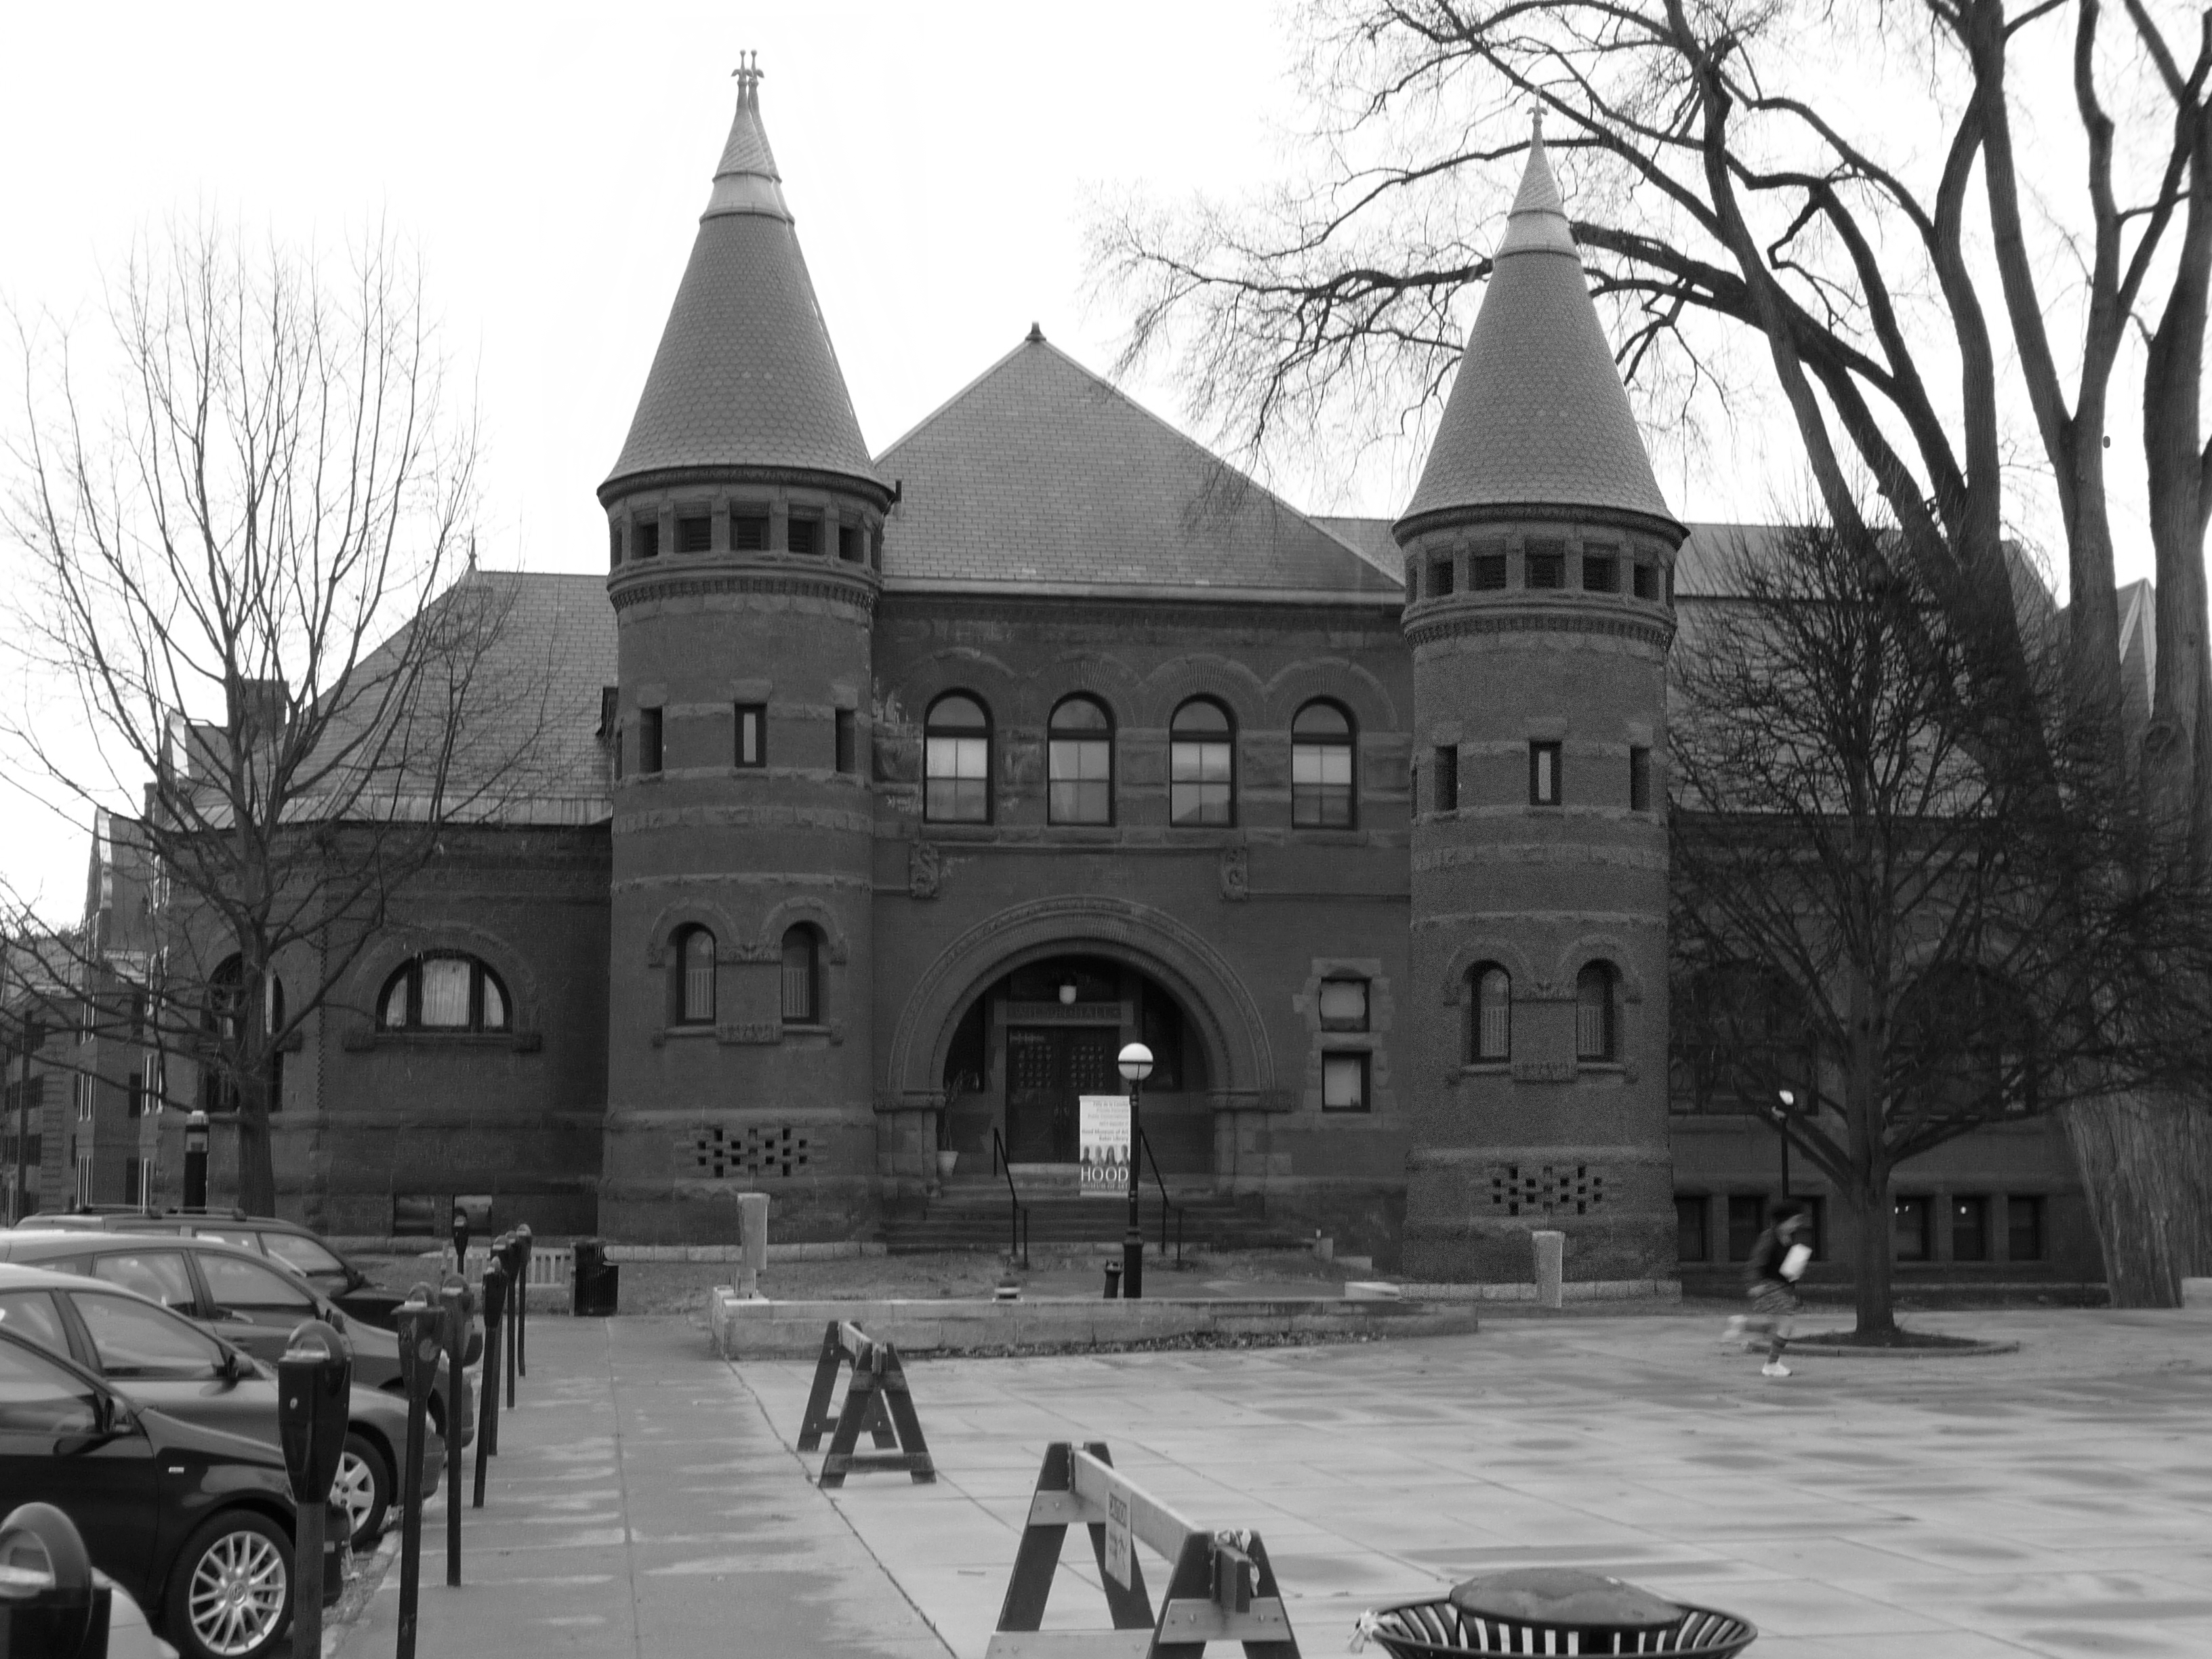
\includegraphics[width=0.45\textwidth]{./images/red_tower.png}}
  \subfigure[Seuil 80]{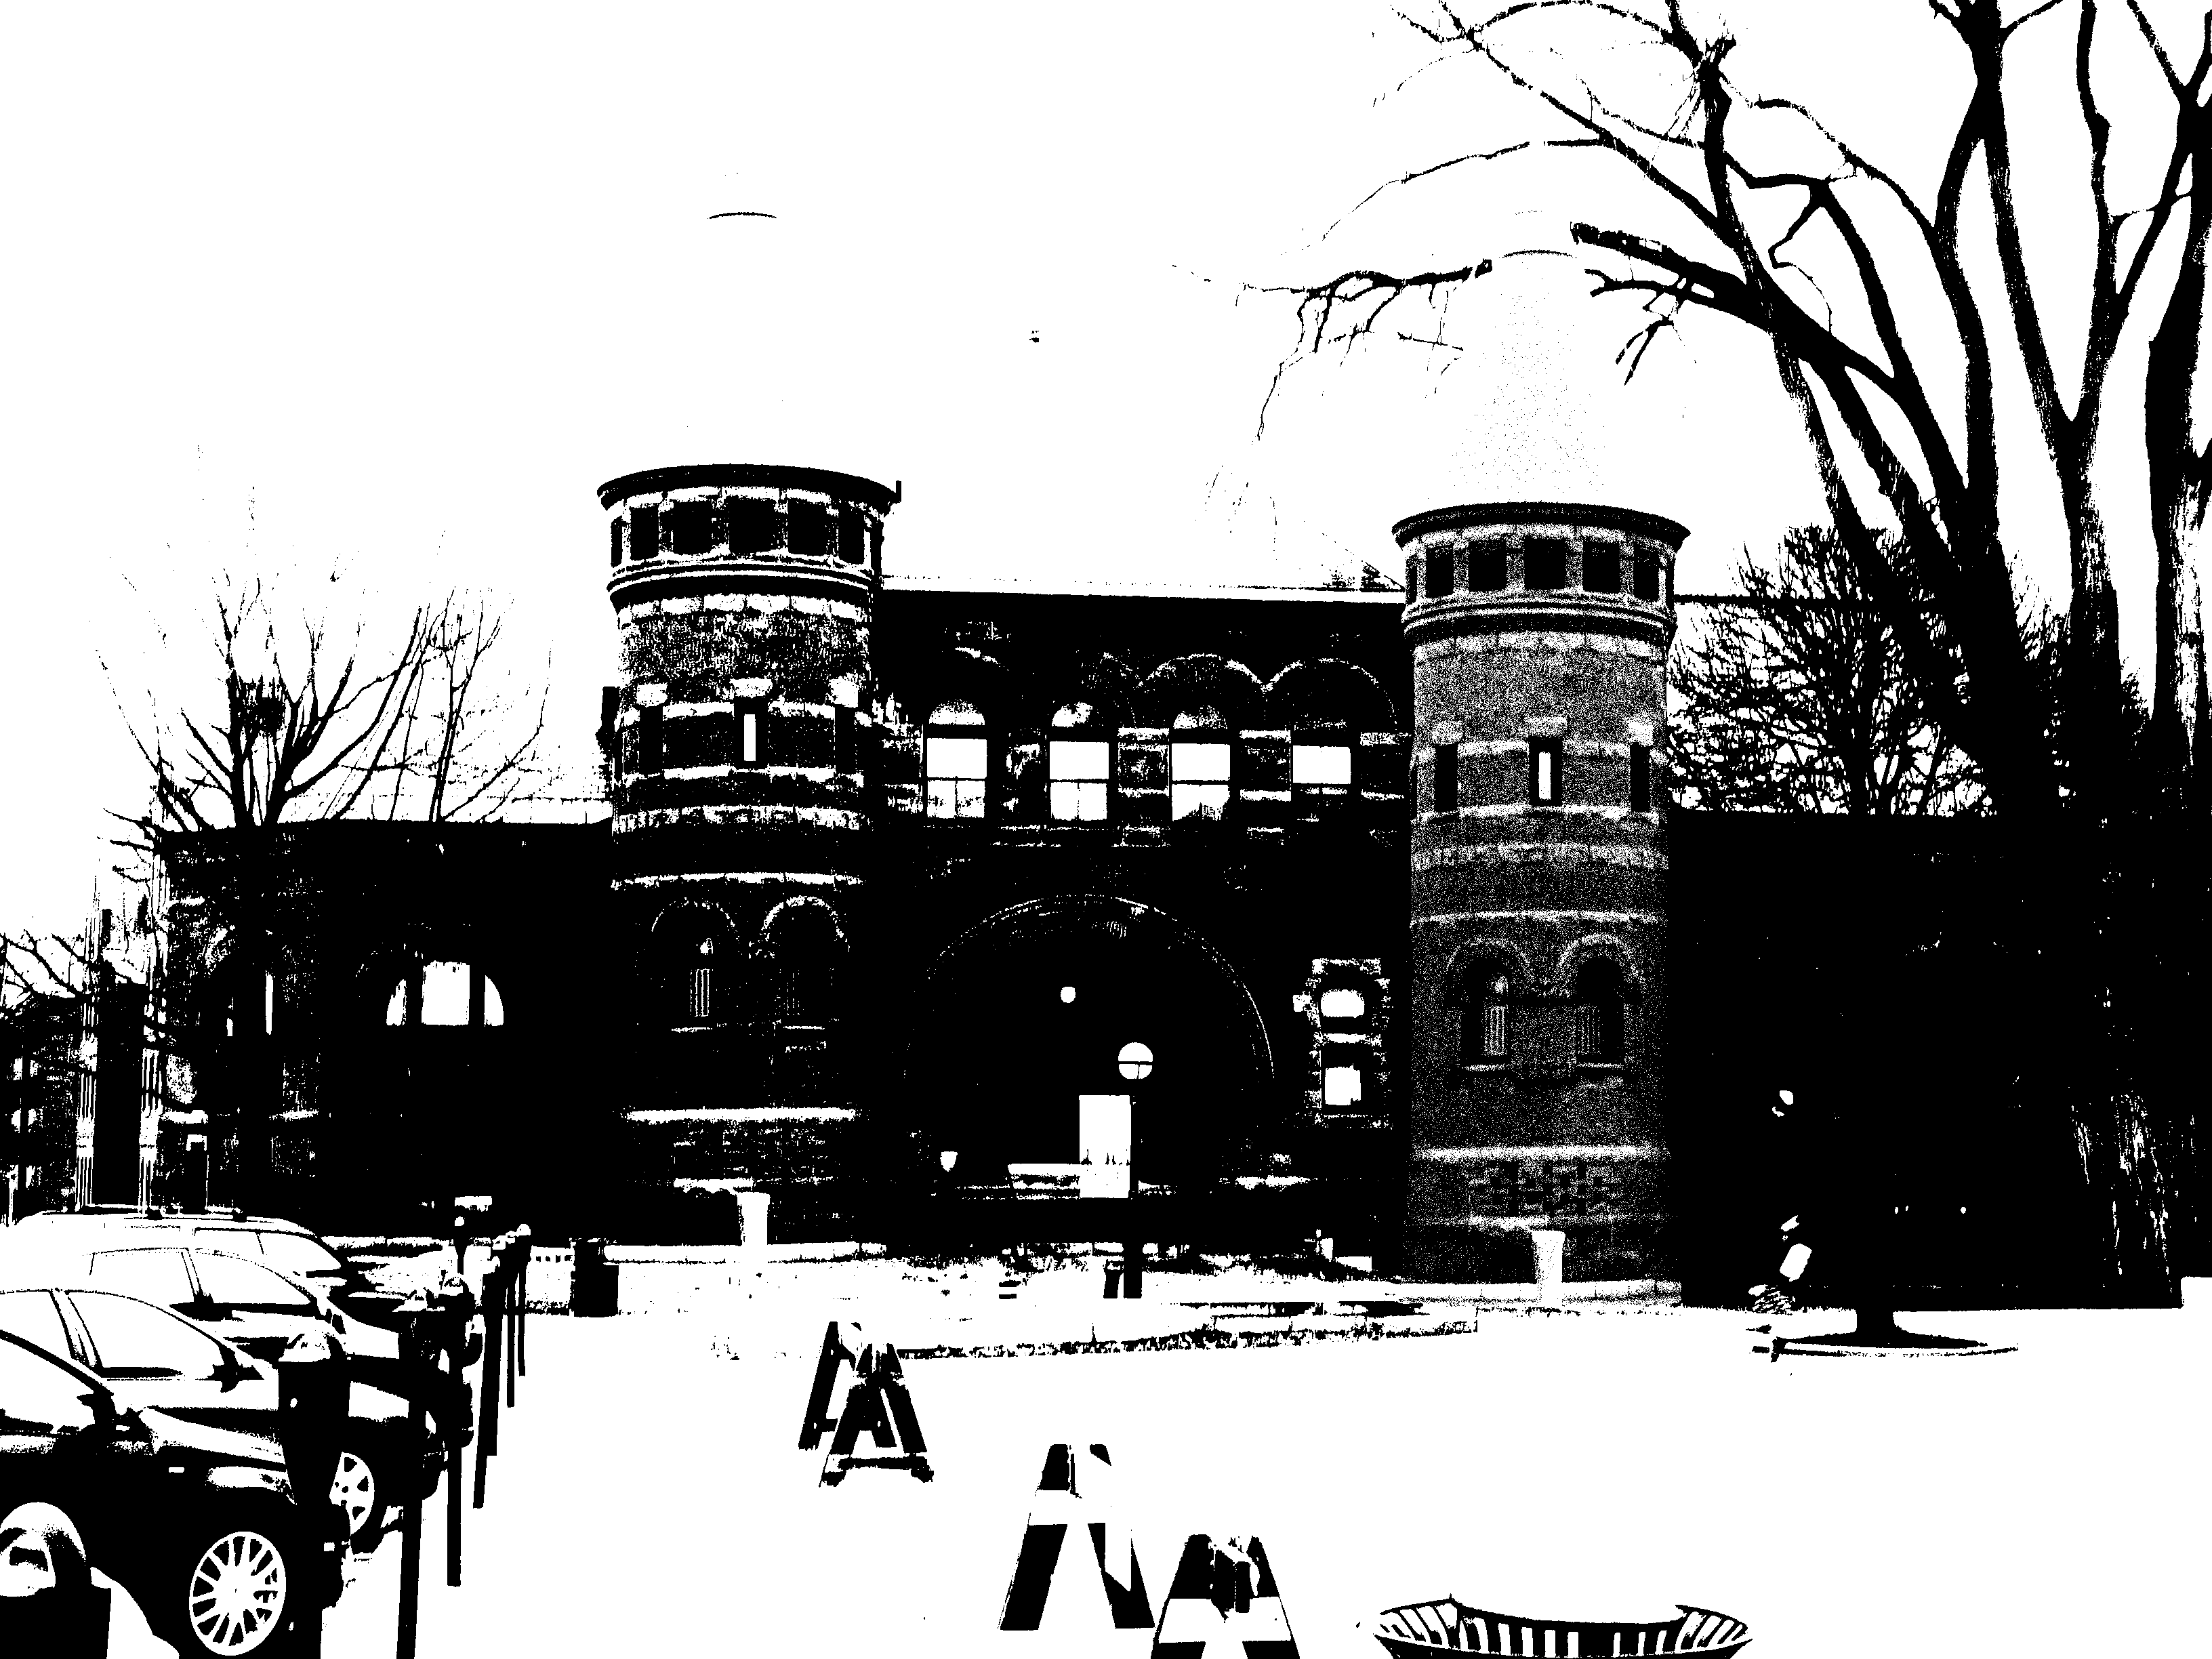
\includegraphics[width=0.45\textwidth]{./images/test_grey1.png}}
  \subfigure[Seuil 150]{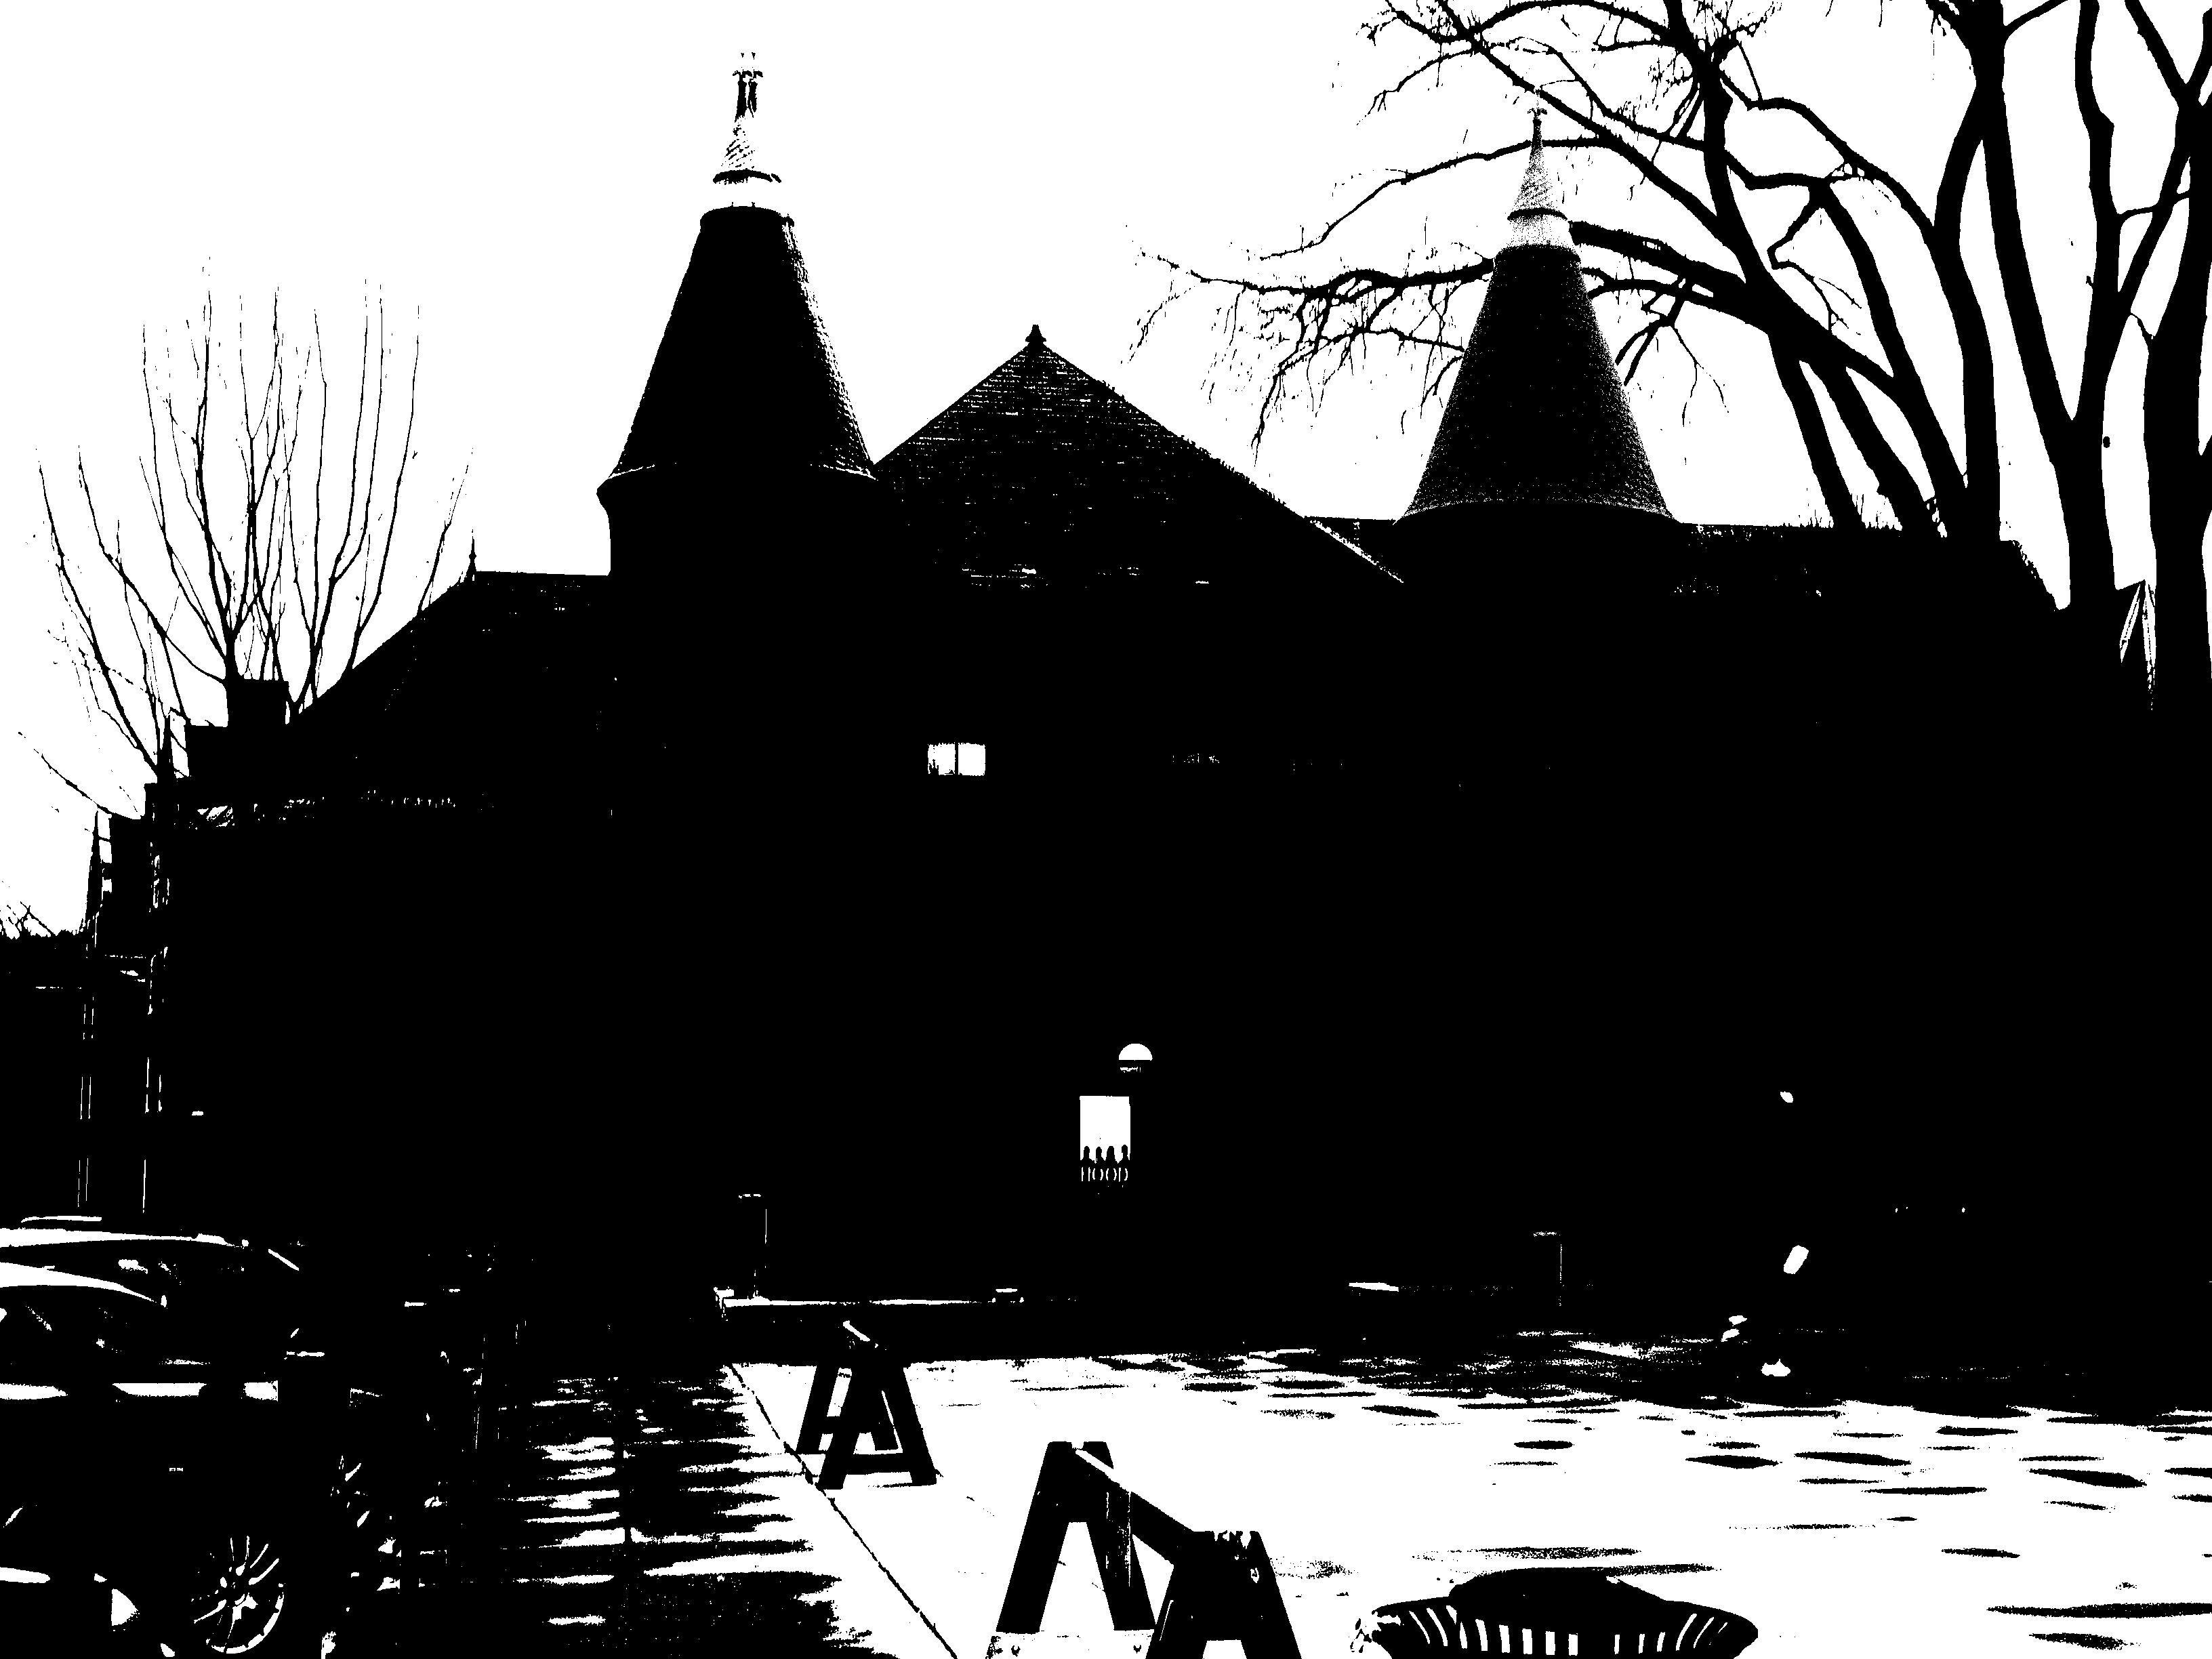
\includegraphics[width=0.45\textwidth]{./images/test_grey2.png}}
  \caption{Résultats}
\end{figure}

\FloatBarrier

\clearpage
\subsection{Seuillage d’une image pgm avec plusieurs niveaux S1, S2, S3}
Cet exercice reprend le programme précédant en y ajoutant un second puis un troisième seuil. Le programme \texttt{test\_grey2.cpp} prend en paramètre 2 seuils. Les pixels dont la valeur est inférieure au premier seuil seront noirs, ceux dont la valeur est comprise entre le premier et le second seront gris et ceux dont la valeur est supérieure au troisième seront blancs. \texttt{test\_grey3.cpp} prend 3 seuils en paramètre, les pixels situés entre deux seuils prendront des valeurs de gris correspondant à une partition égale de 256 en 4 parties.

\begin{figure}[!htb]
  \centering
  \subfigure[Image originale]{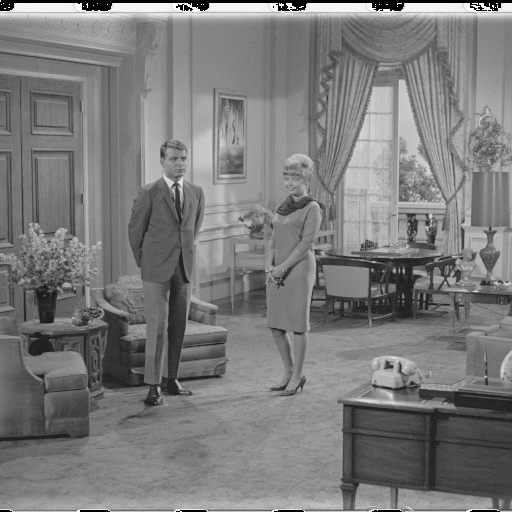
\includegraphics[width=0.35\textwidth]{./images/couple.png}}
  \subfigure[Seuils 50 120]{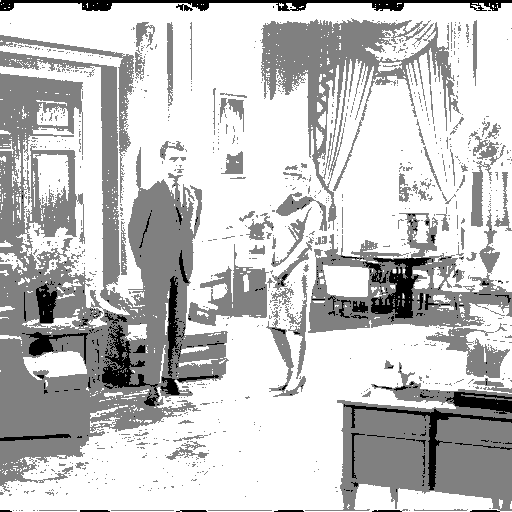
\includegraphics[width=0.35\textwidth]{./images/test_grey_2_1.png}}
  \subfigure[Seuils 80 200]{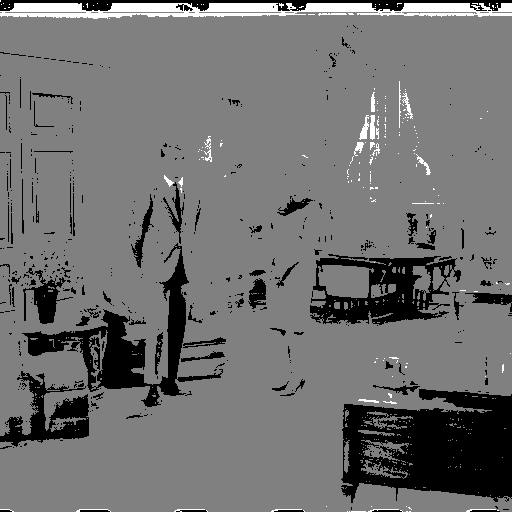
\includegraphics[width=0.35\textwidth]{./images/test_grey_2_2.png}}
  \subfigure[Seuils 50 120 200]{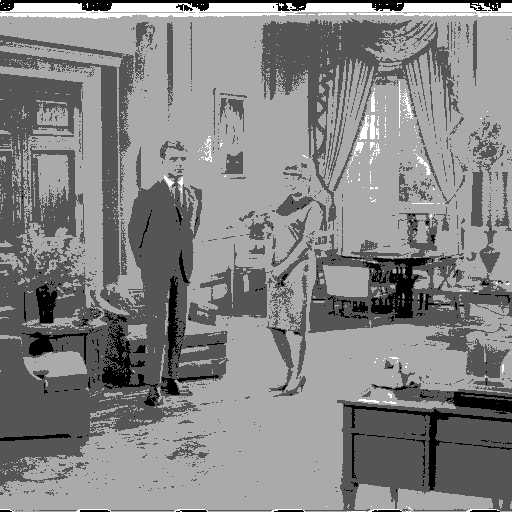
\includegraphics[width=0.35\textwidth]{./images/test_grey_3_1.png}}
  \caption{Résultats}
\end{figure}

\FloatBarrier

\clearpage
\subsection{Histogramme d'une image pgm}
Cet exercice consiste à créer un programme \texttt{histo.cpp} qui affiche l'histogramme d'une image. L'histogramme est un tableau de 256 cases, chaque case correspondant à une valeur de pixel. Le programme lit l'image et compte le nombre de pixels de chaque valeur. Il écrit ensuite le résultat dans un fichier \texttt{histo.dat} que l'on affiche avec \texttt{gnuplot}.

\begin{figure}[!htb]
  \centering
  \subfigure[Image originale]{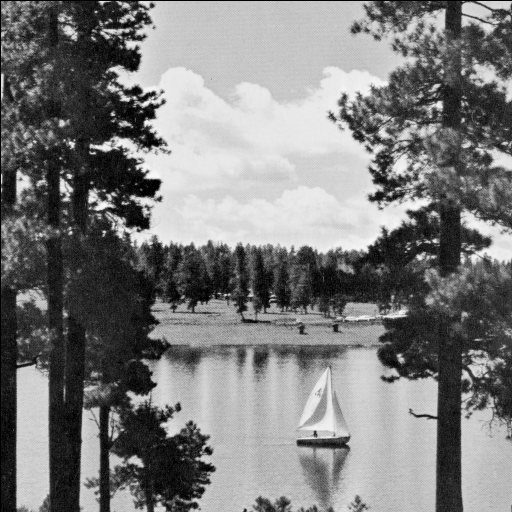
\includegraphics[width=0.5\textwidth]{./images/sailboat.png}}
  \subfigure[Histogramme généré]{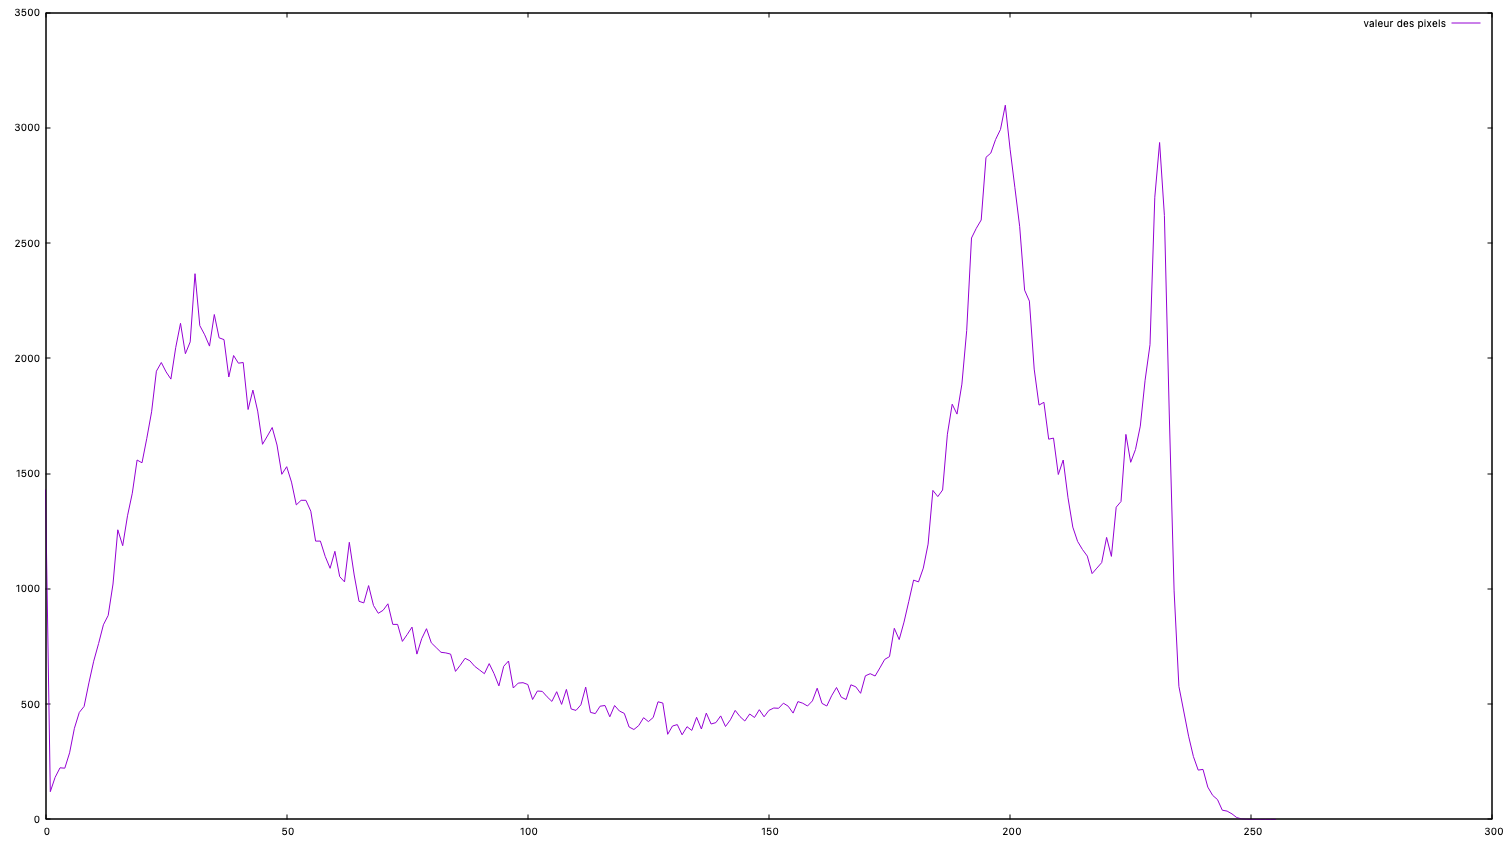
\includegraphics[width=0.8\textwidth]{./images/histo.png}}
  \caption{Résultats}
\end{figure}

\FloatBarrier

\clearpage
\subsection{Profil d'une ligne ou d'une colonne d'une image pgm}
Cet exercice consiste à créer un programme \texttt{profil.cpp} qui affiche le profil d'une ligne ou d'une colonne d'une image. Le programme lit une ligne ou une colonne de l'image et store la valeur des pixels. Il écrit ensuite le résultat dans un fichier \texttt{profil.dat} que l'on affiche avec \texttt{gnuplot}.

\begin{figure}[!htb]
  \centering
  \subfigure[Image originale]{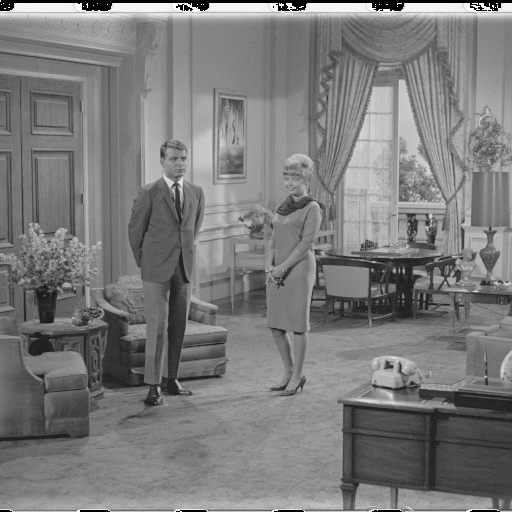
\includegraphics[width=0.5\textwidth]{./images/couple.png}}
  \subfigure[Histogramme généré pour la ligne 150]{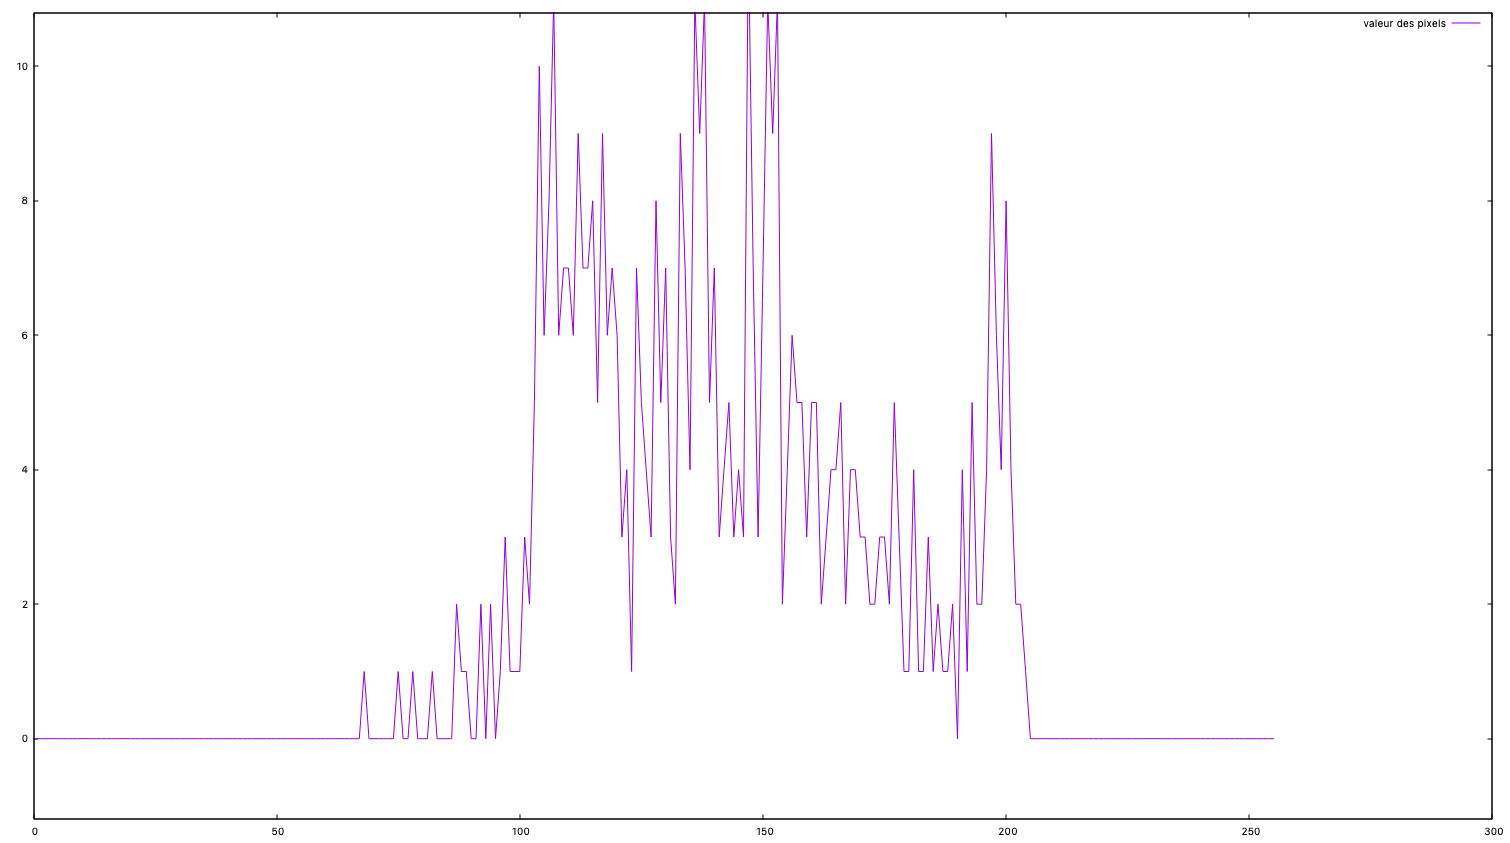
\includegraphics[width=0.8\textwidth]{./images/profil.png}}
  \caption{Résultats}
\end{figure}

\FloatBarrier

\clearpage
\subsection{Seuillage d’une image couleur}
De manière similaire à l'exercice 2, cet exercice consiste à créer un programme \texttt{test\_couleur.cpp} qui prend en paramètre 3 seuils. Pour chaque composante, R, G et B, les pixels dont la valeur est inférieure au premier seuil seront noirs et ceux dont la valeur est supérieure au troisième seront respectivement rouges,verts ou bleus.

\begin{figure}[!htb]
  \centering
  \subfigure[Image originale]{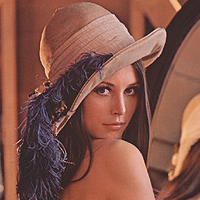
\includegraphics[width=0.45\textwidth]{./images/lena.png}}
  \subfigure[Seuils 80 50 100]{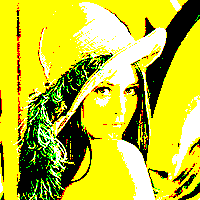
\includegraphics[width=0.45\textwidth]{./images/test_couleur1.png}}
  \subfigure[Seuils 120 180 100]{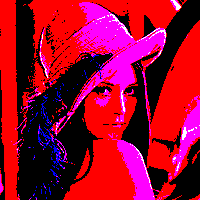
\includegraphics[width=0.45\textwidth]{./images/test_couleur2.png}}
  \caption{Résultats}
\end{figure}

\FloatBarrier

\clearpage
\subsection{Histogrammes des 3 composantes d'une image couleur}
À la manière de l'exercice 3, cet exercice consiste à créer un programme \texttt{histo\_rgb.cpp} qui affiche l'histogramme des 3 composantes d'une image couleur. Le programme lit l'image et compte le nombre de pixels de chaque valeur pour chaque composante. Il écrit ensuite le résultat dans un fichier \texttt{histo\_rgb.dat} que l'on affiche avec \texttt{gnuplot}.


\begin{figure}[!htb]
  \centering
  \subfigure[Image originale]{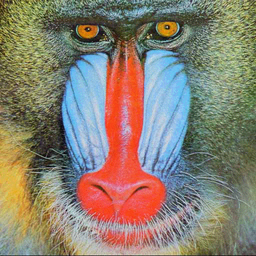
\includegraphics[width=0.5\textwidth]{./images/baboon.png}}
  \subfigure[Histogramme généré]{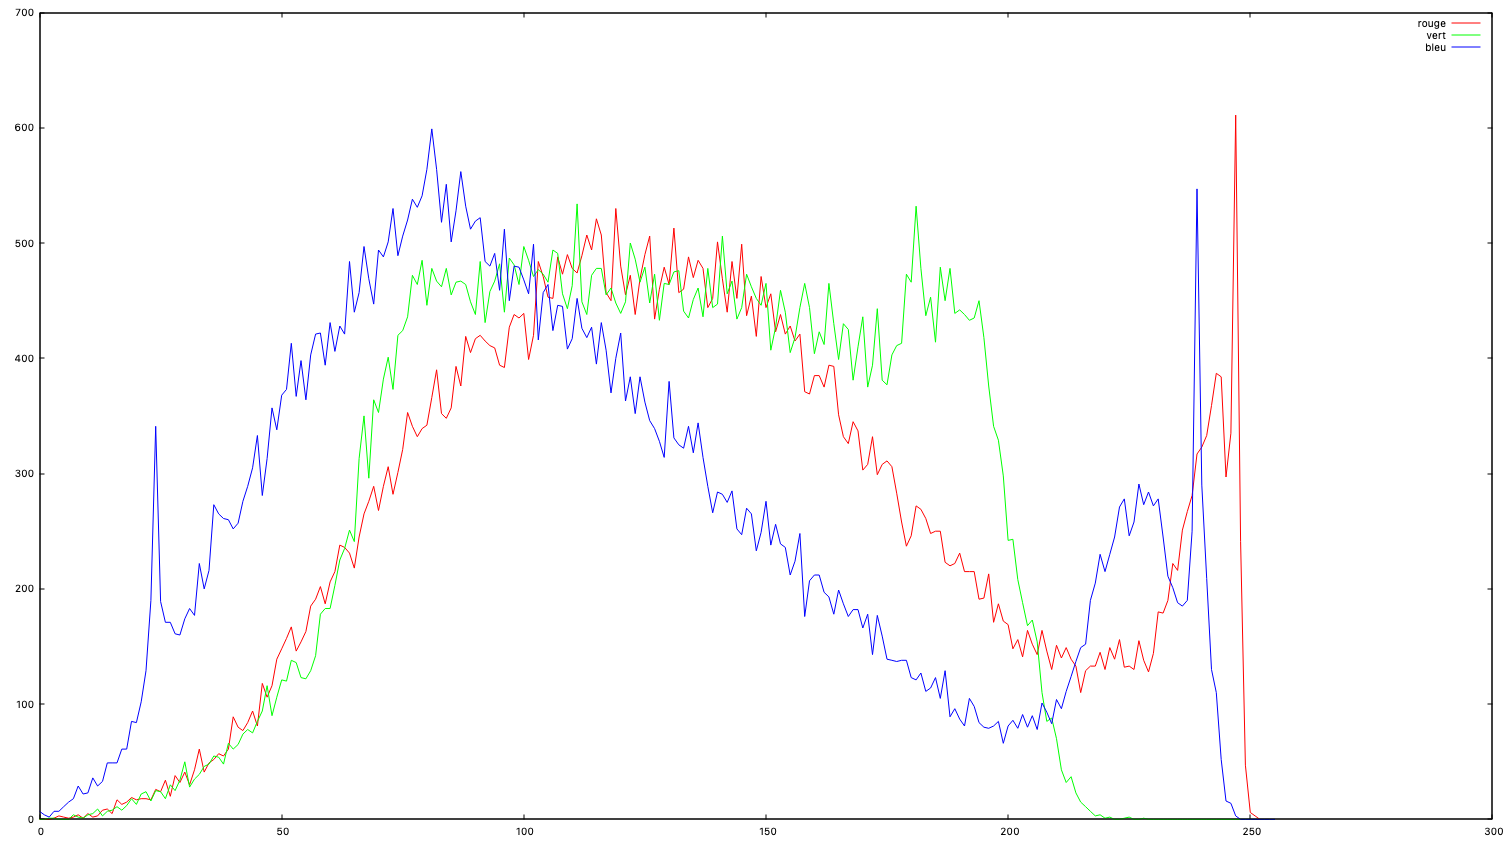
\includegraphics[width=0.8\textwidth]{./images/histo_rgb.png}}
  \caption{Résultats}
\end{figure}

\FloatBarrier

\clearpage
\section{Exercices facultatifs}
\subsection{Correction Gamma}
Cet exercice consiste à créer un programme \texttt{gamma.cpp} qui applique une correction gamma à une image, qui se rapproche d'une correction de contraste. Le programme lit l'image et applique la formule V\textsubscript{\text{out}}=AV\textsubscript{\text{in}}\textsuperscript{\(\gamma\) } à chaque pixel.

J'ai réalisé le programme à la fois pour les images pgm et ppm, avec une seule valeur ou une par composante, ainsi qu'un histogramme afin de visualiser la courbe de correction gamma.

\begin{figure}[!htb]
  \centering
  \subfigure[Courbe pour gamma = 1.8]{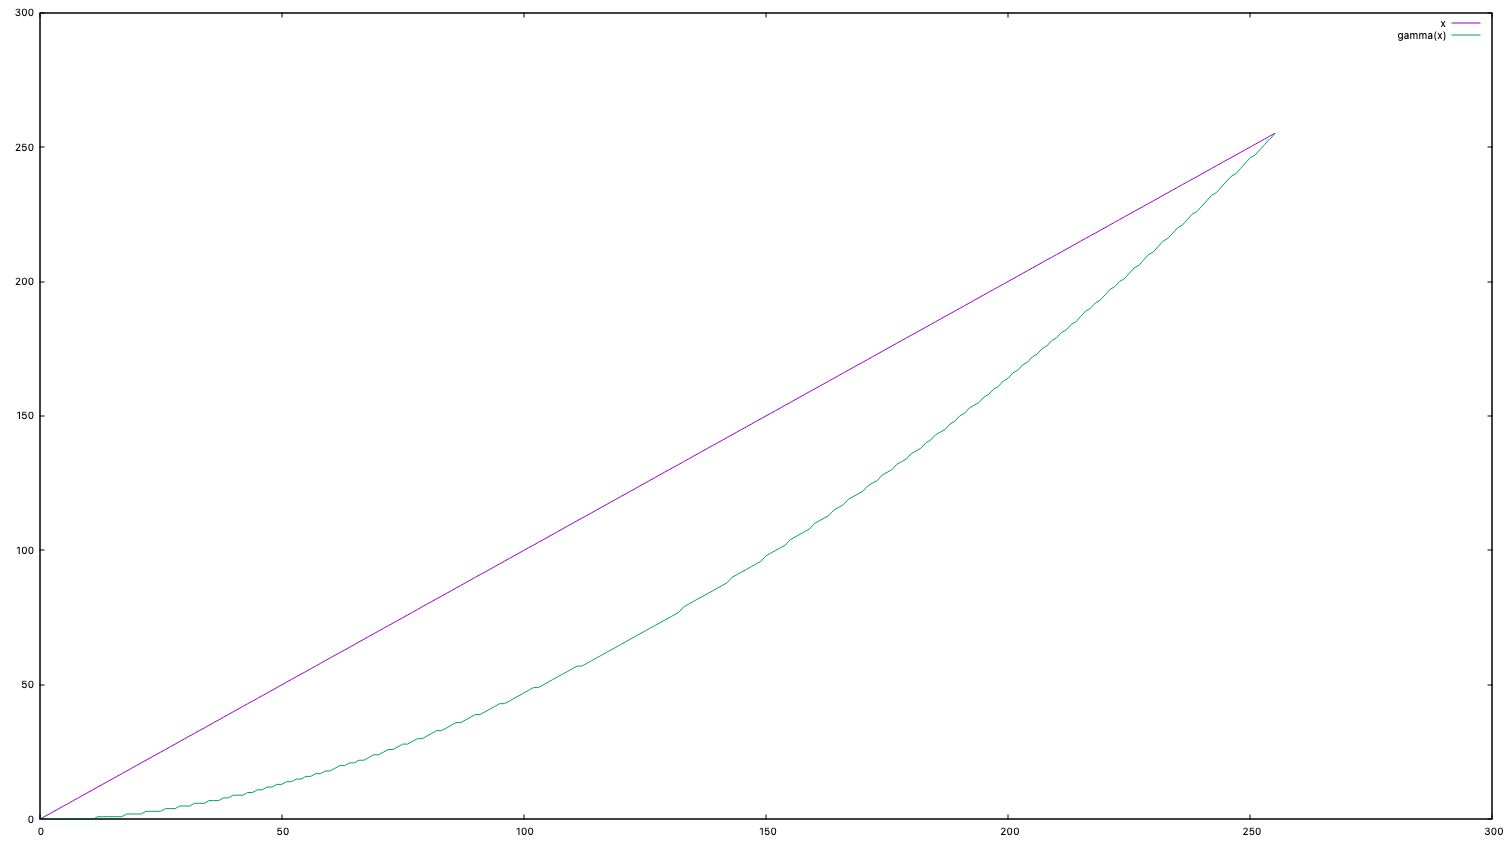
\includegraphics[width=0.8\textwidth]{./images/gamma_curve_1_8.png}}
  \subfigure[Courbe pour gamma = 0.6]{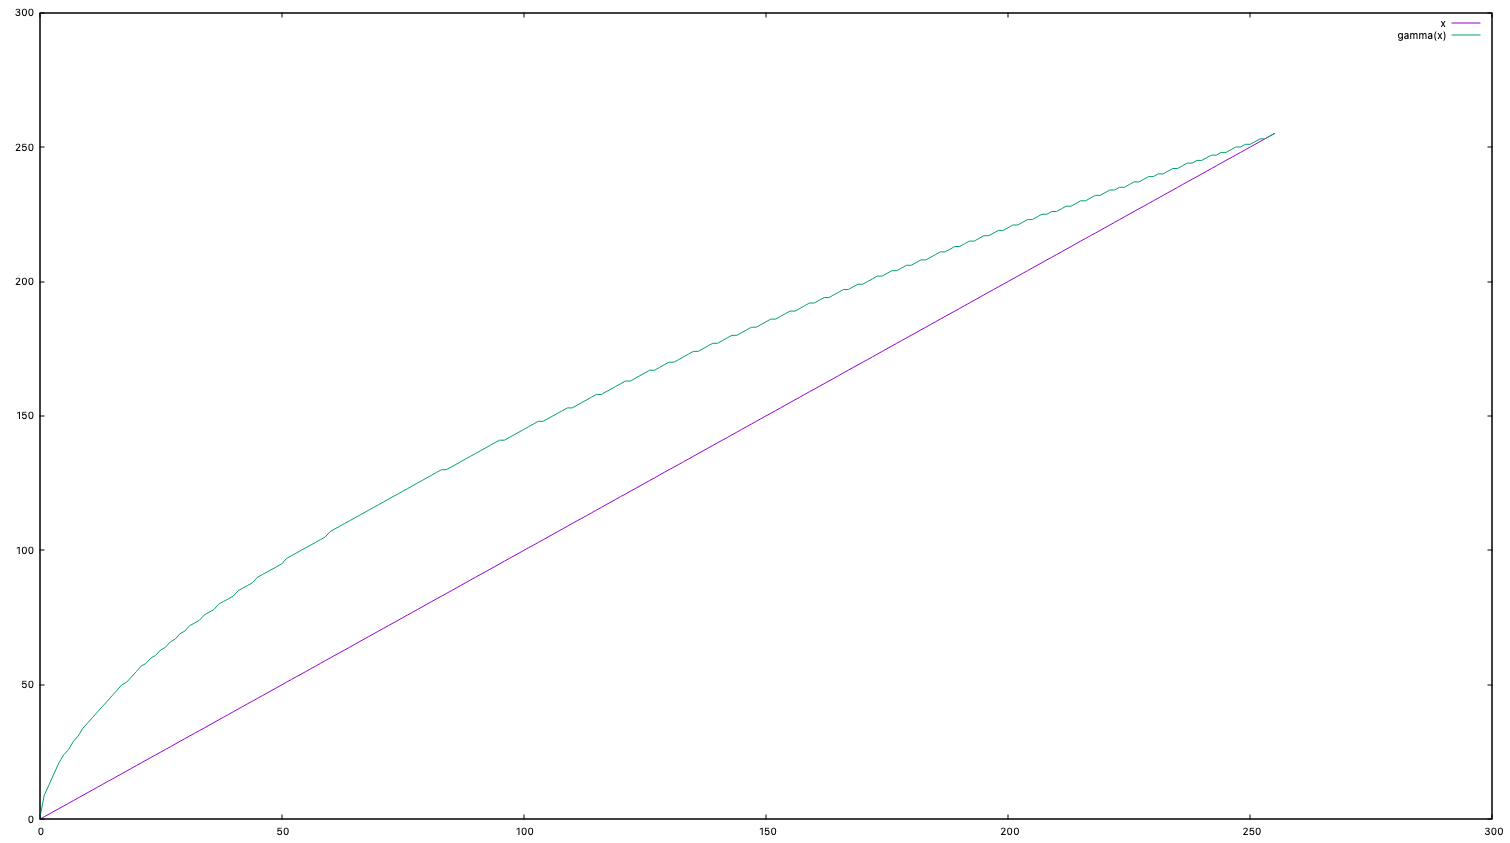
\includegraphics[width=0.8\textwidth]{./images/gamma_curve_0_6.png}}
  \caption{Courbes}
\end{figure}


\begin{figure}[!htb]
  \centering
\subfigure[Image originale]{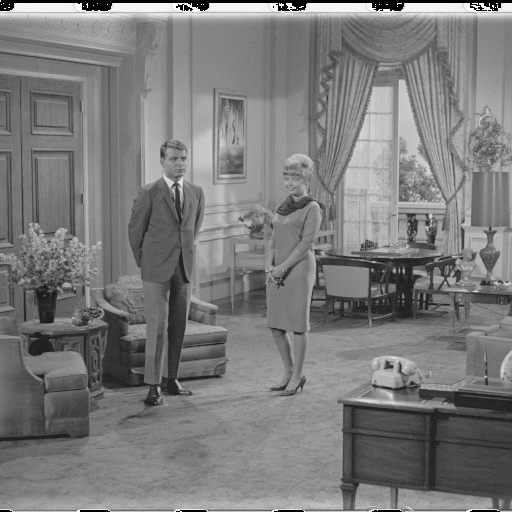
\includegraphics[width=0.45\textwidth]{./images/couple.png}}
\subfigure[Gamma = 1.8]{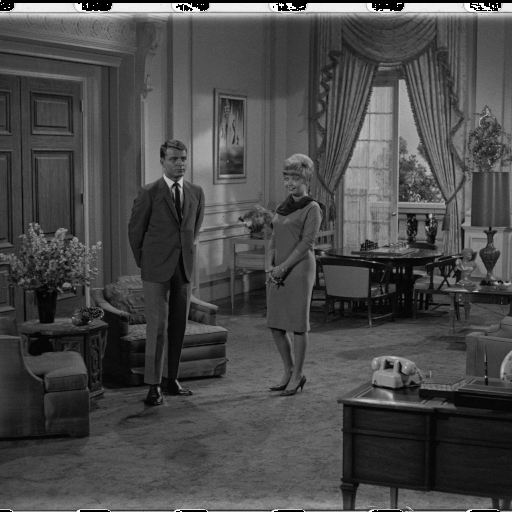
\includegraphics[width=0.45\textwidth]{./images/gamma1.png}}
\subfigure[Gamma = 0.6]{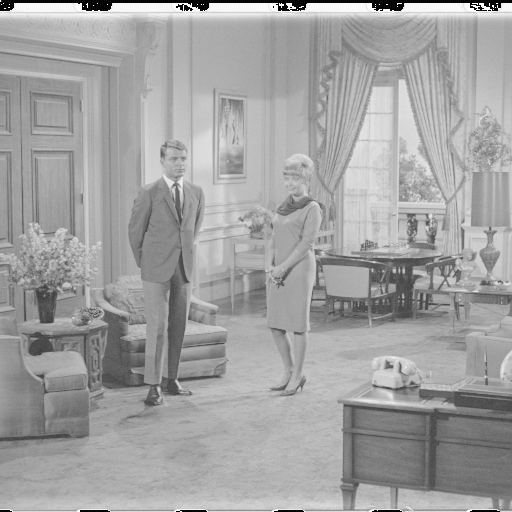
\includegraphics[width=0.45\textwidth]{./images/gamma2.png}}
  \caption{Correction sur une image pgm}
\end{figure}


\begin{figure}[!htb]
  \centering
\subfigure[Image originale]{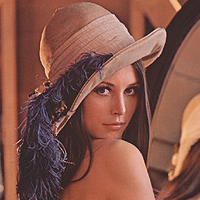
\includegraphics[width=0.35\textwidth]{./images/lena.png}}
\subfigure[Gamma = 1.8]{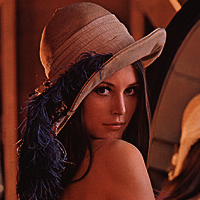
\includegraphics[width=0.35\textwidth]{./images/gamma_rgb1.png}}
\subfigure[Gamma = 0.6]{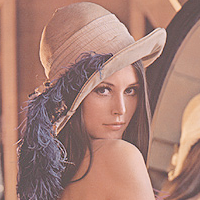
\includegraphics[width=0.35\textwidth]{./images/gamma_rgb2.png}}
\subfigure[Gamma = \{1.8, 0.8, 2.2\}]{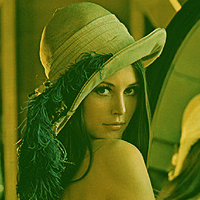
\includegraphics[width=0.35\textwidth]{./images/gamma_rgb_multi.png}}
\caption{Correction sur une image ppm}
\end{figure}

\FloatBarrier

\clearpage
\subsection{Seuillage avec un nombre inconnu de seuils}
Tout comme l'exercice 2, cet exercice consiste à créer un programme \texttt{seuil\_x.cpp}  qui prend en paramètre un nombre \texttt{x} de seuils. Il calcule ensuite les valeurs qui seront appliquées aux pixels en fonction de leur valeur. Les pixels dont la valeur est inférieure au premier seuil seront noirs, ceux dont la valeur est supérieure au dernier seront blancs et ceux dont la valeur est comprise entre deux seuils prendront une nuance de gris.

\begin{figure}[!htb]
  \centering
  \subfigure[Image originale]{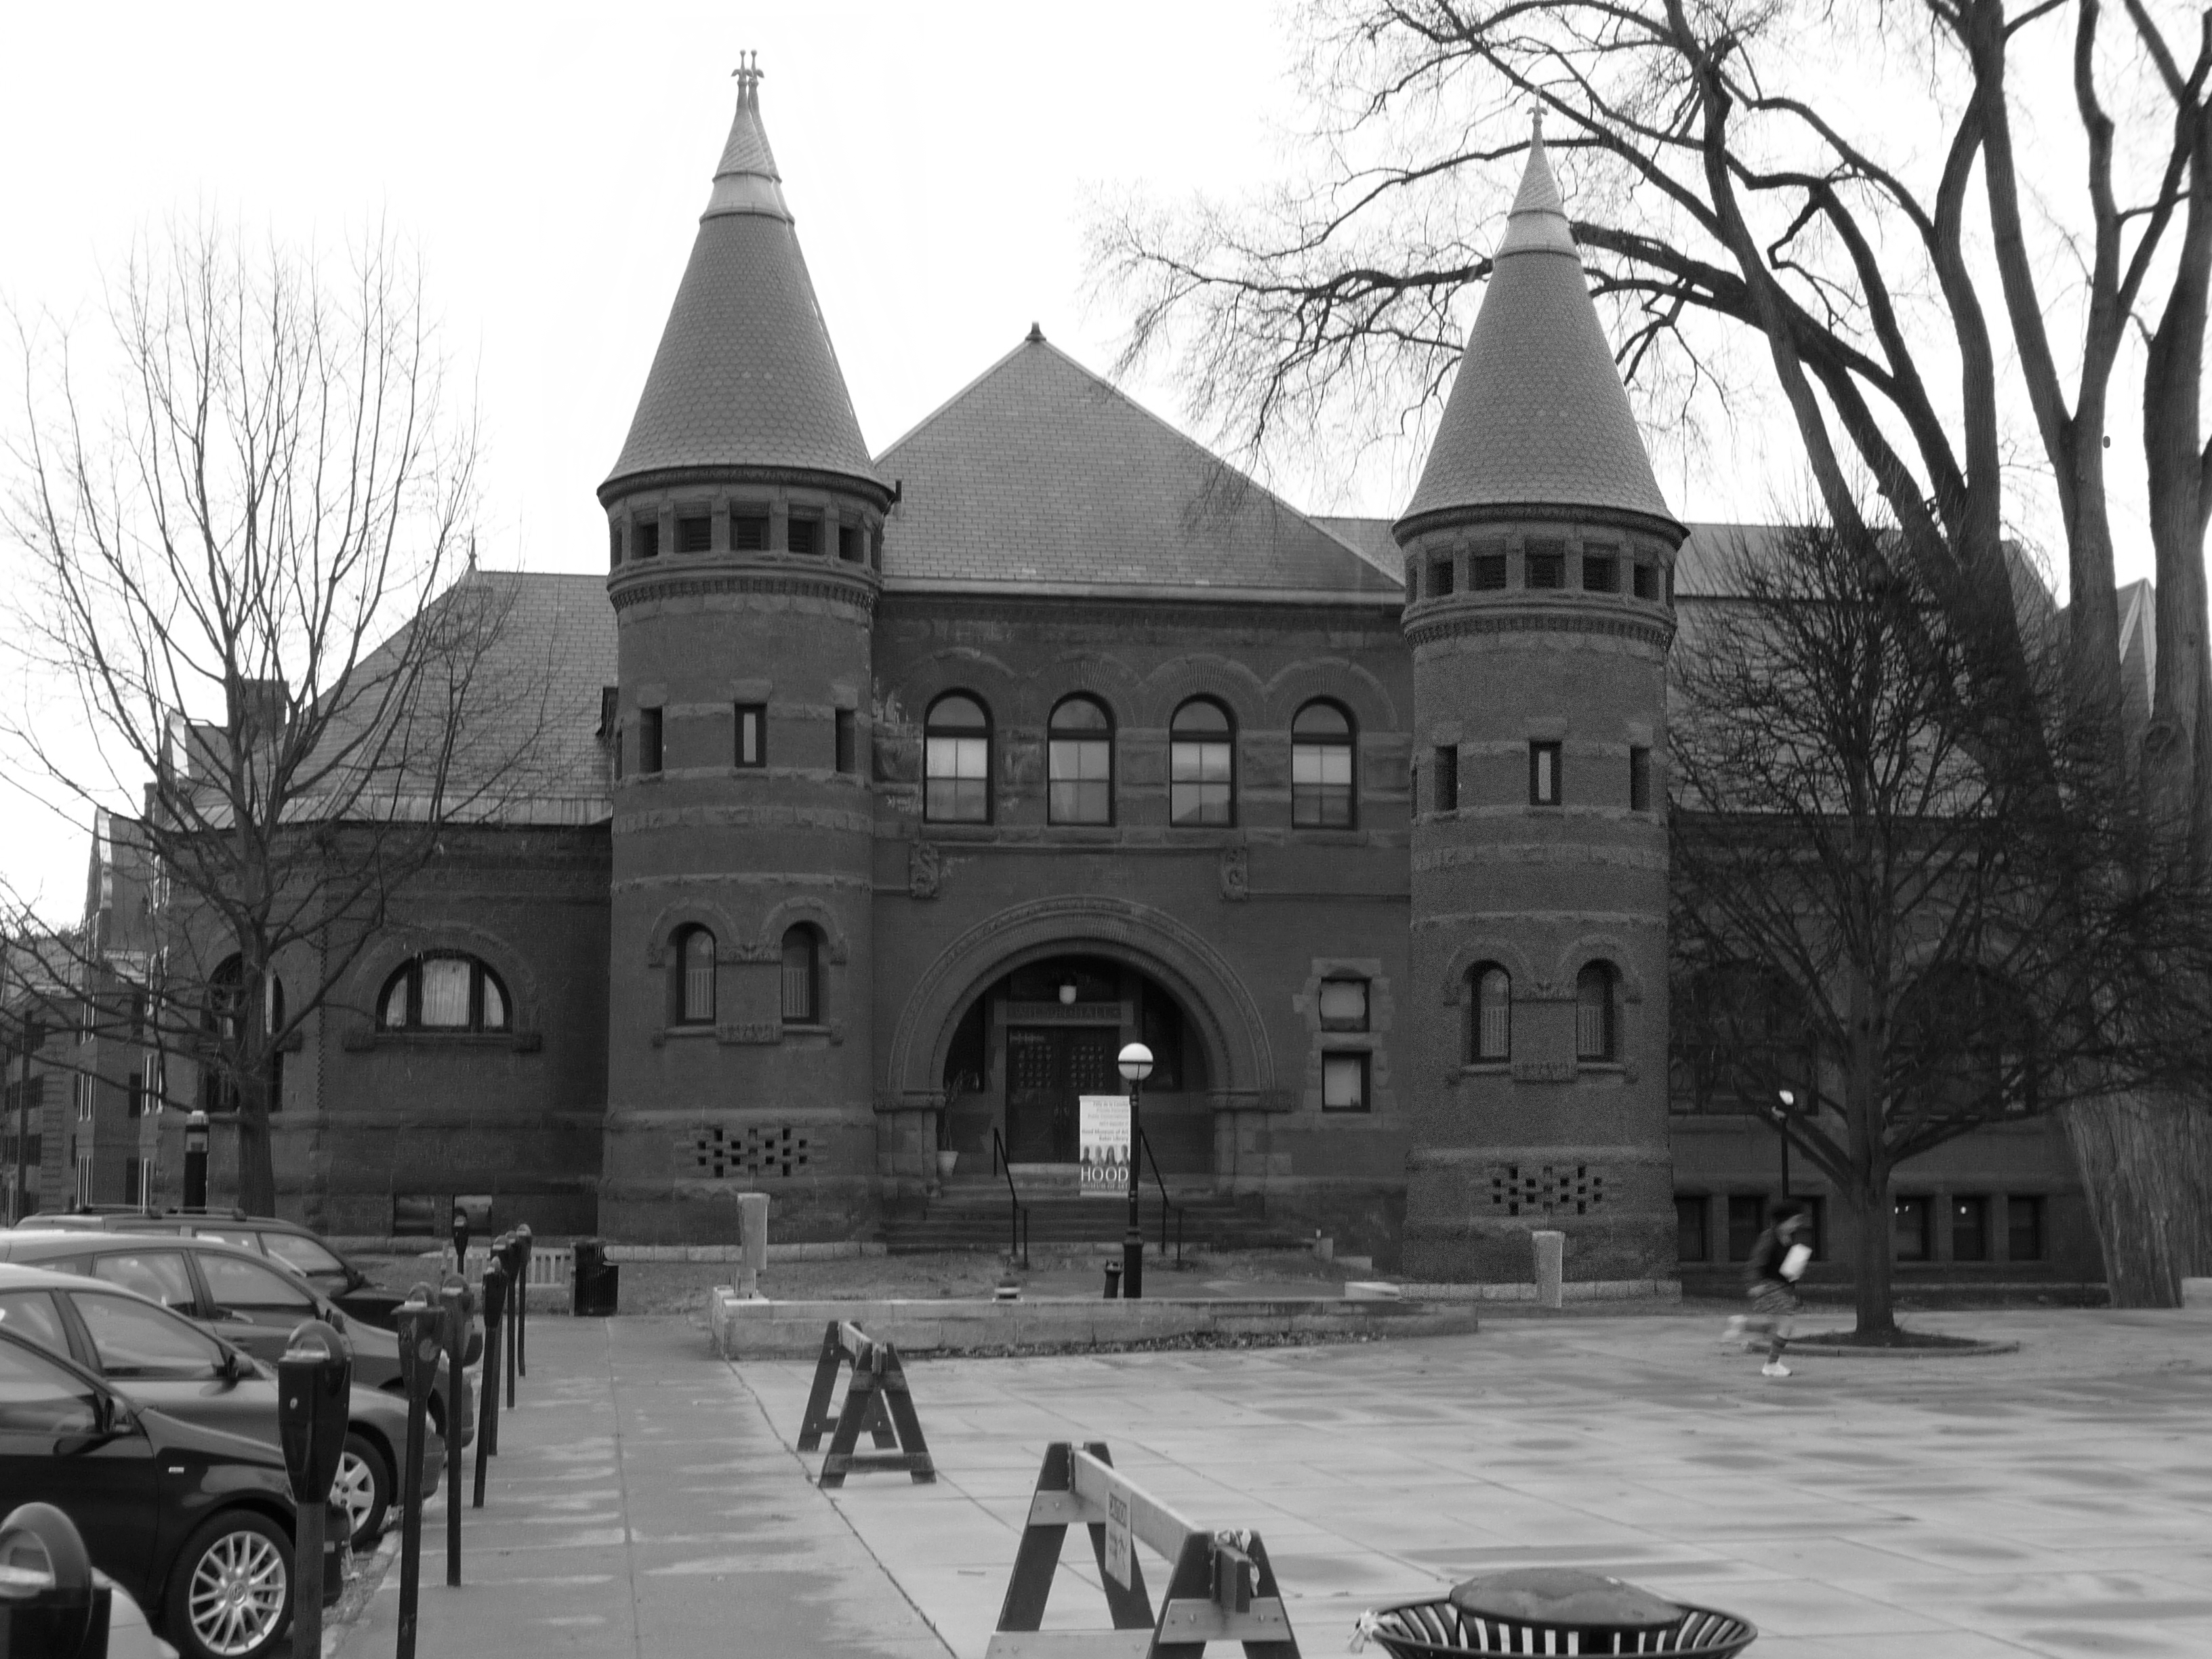
\includegraphics[width=0.65\textwidth]{./images/red_tower.png}}
  \subfigure[Seuils 10 50 128 132 200 220]{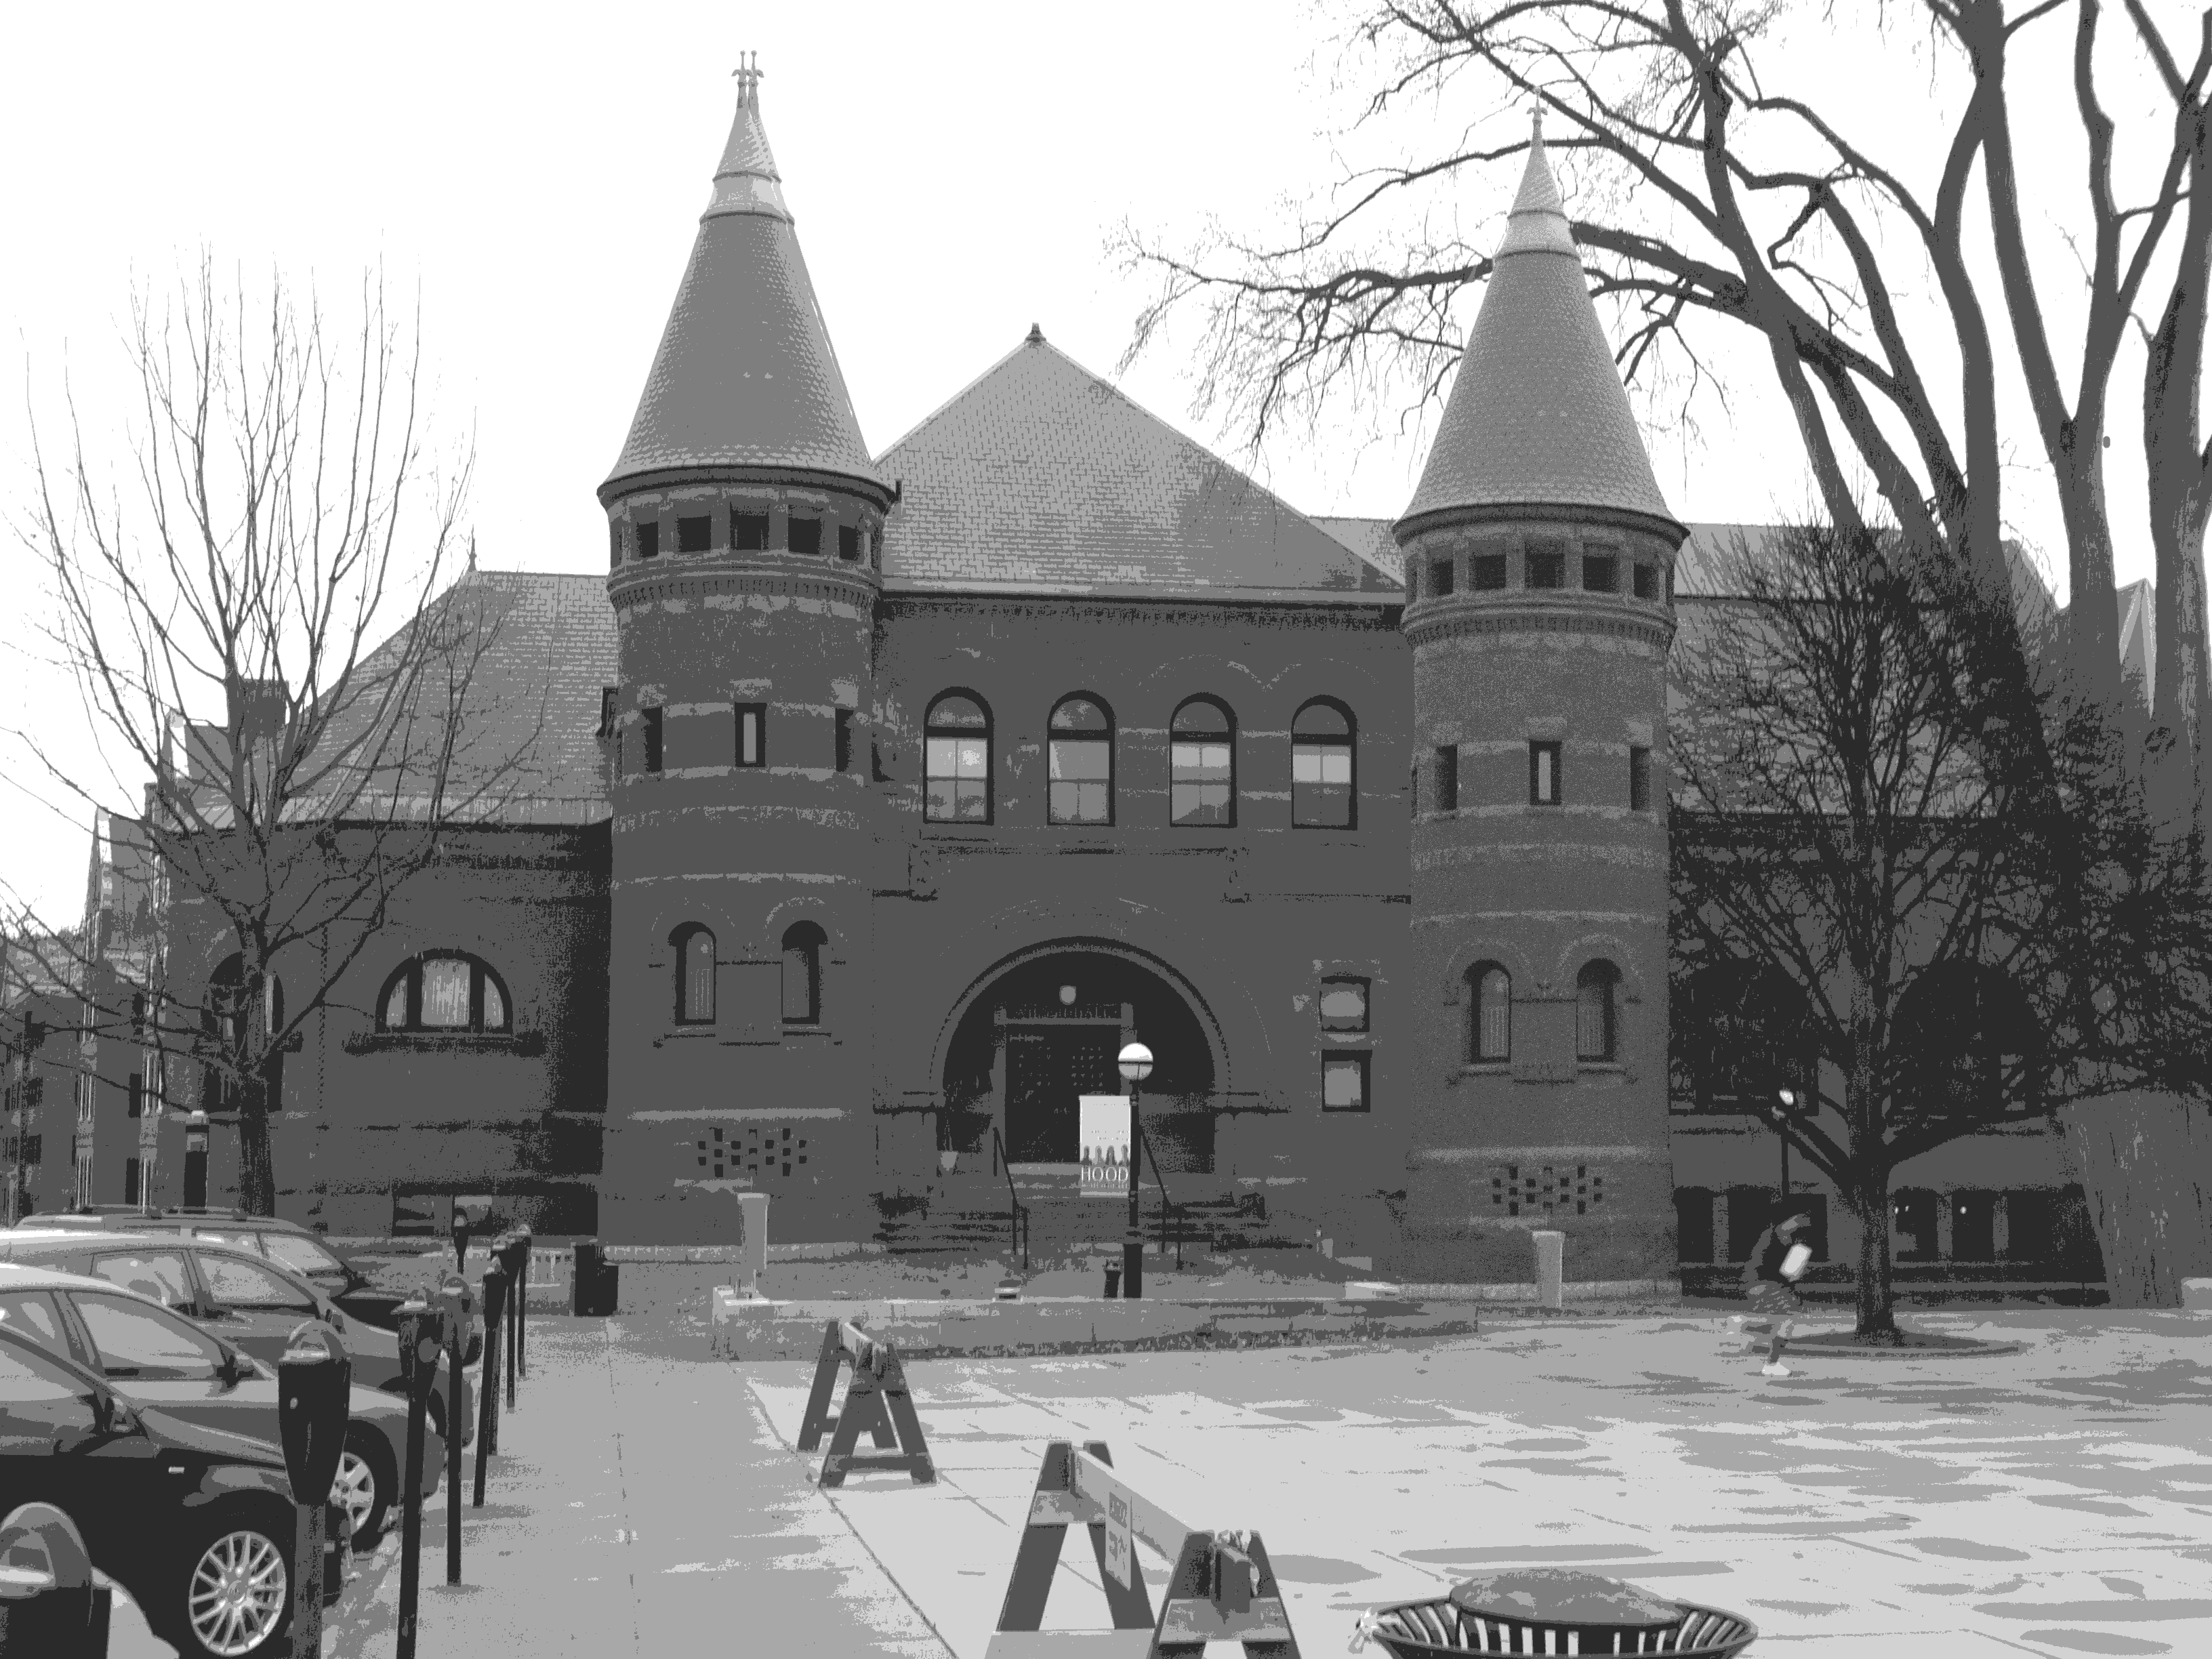
\includegraphics[width=0.65\textwidth]{./images/seuil_x.png}}
  \caption{Résultats}
\end{figure}
 
\FloatBarrier

\clearpage
\subsection{Interpolation entre 2 seuils}
Cet exercice consiste à realiser une interpolation linéaire de manière à ce que les pixels dont la valeur est comprise entre deux seuils prennent une nuance de gris. Le programme \texttt{interpolation.cpp} prend en paramètre 2 seuils. Les pixels dont la valeur est inférieure au premier seuil seront noirs, ceux dont la valeur est supérieure au second seront blancs et ceux dont la valeur est comprise entre les deux prendront une nuance de gris selon une fonction, soit affine, soit sinusoïdale.

\begin{figure}[!htb]
  \centering
  \subfigure[Courbes d'interpolation]{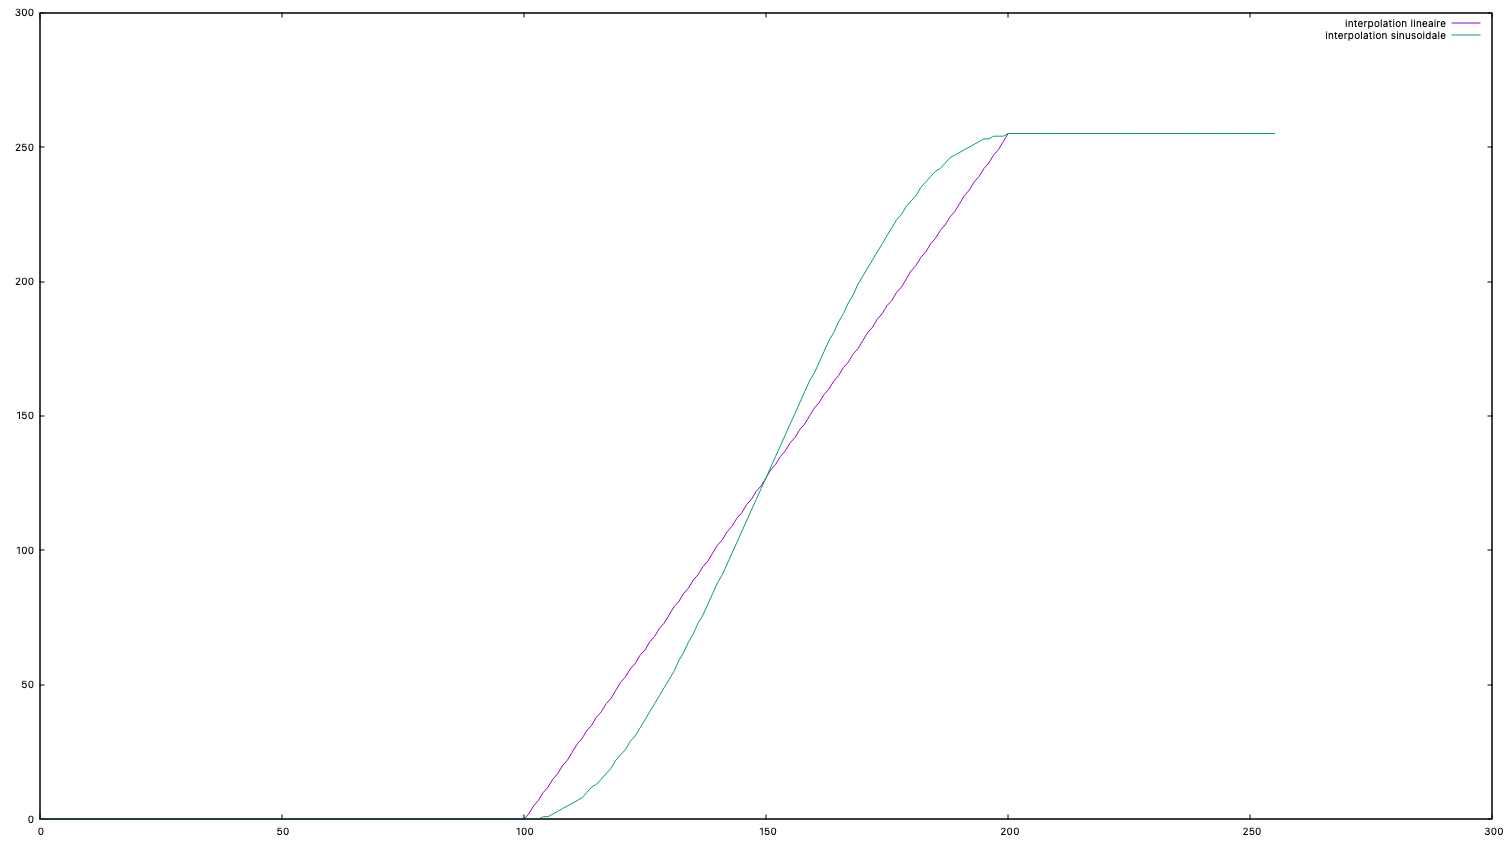
\includegraphics[width=0.8\textwidth]{./images/interpolation_curve.png}}
  \subfigure[Image originale]{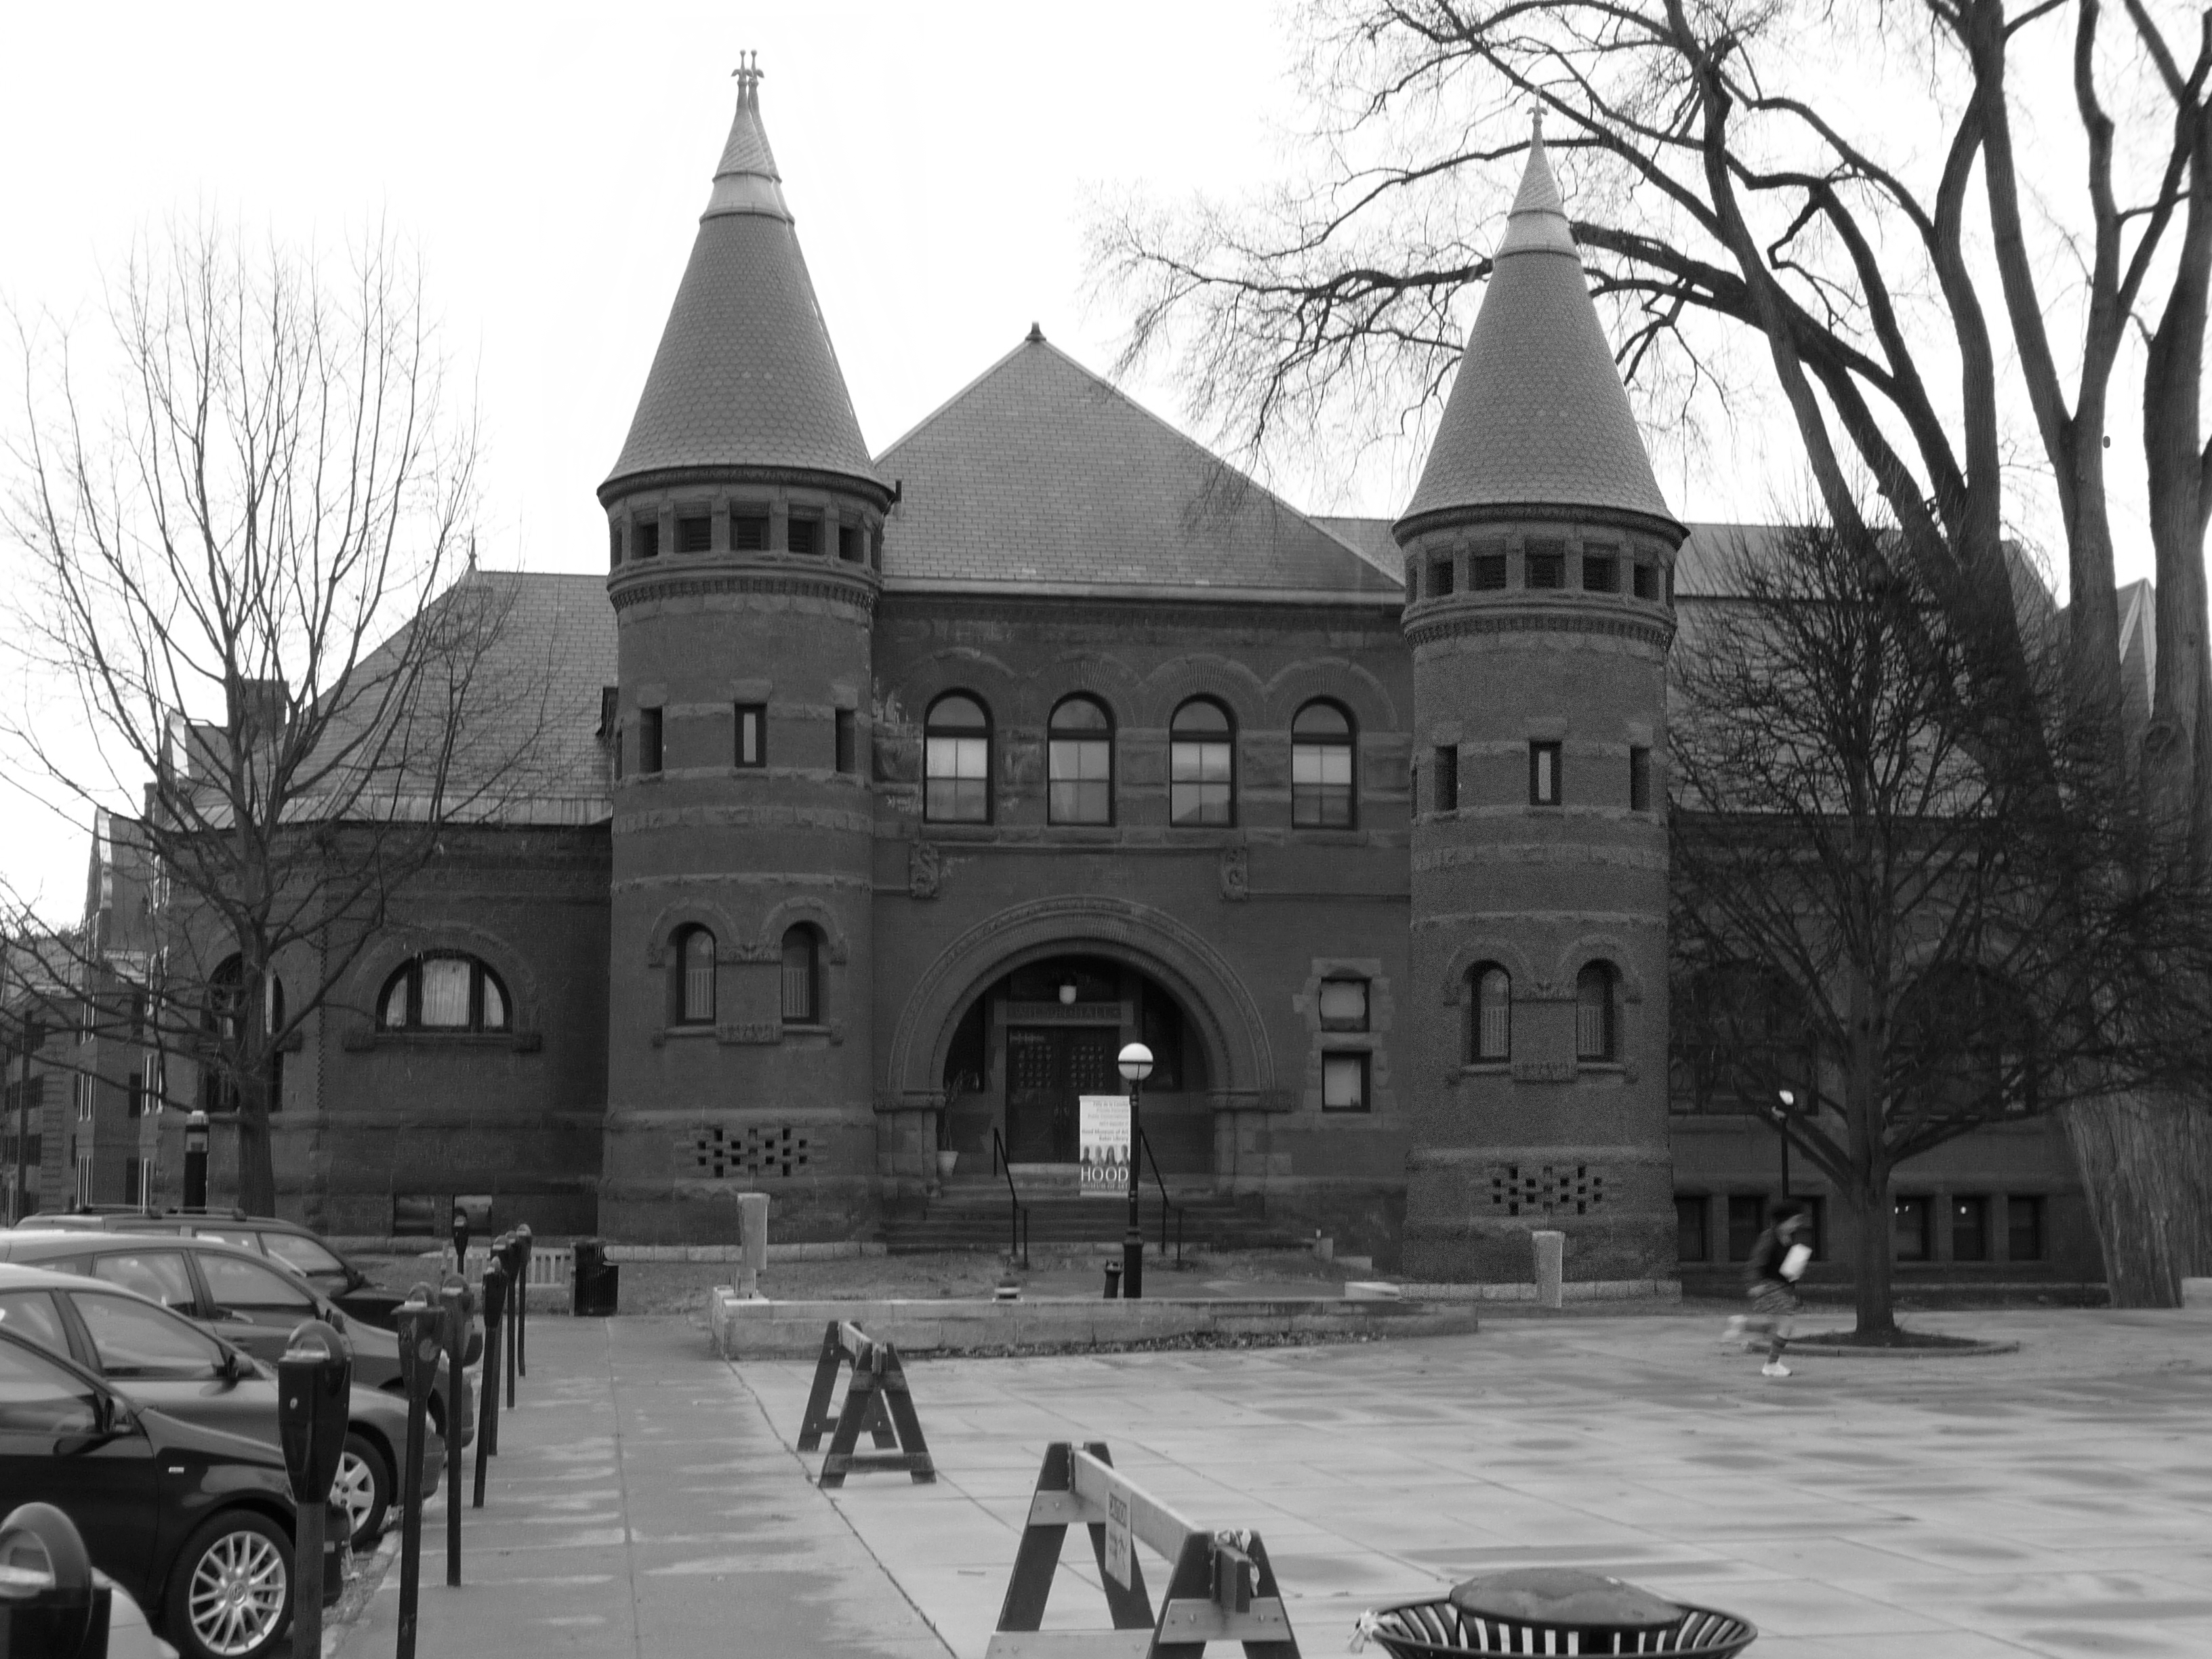
\includegraphics[width=0.5\textwidth]{./images/red_tower.png}}
\end{figure}
\clearpage
\begin{figure}[!htb]
  \subfigure[Interpolation linéaire]{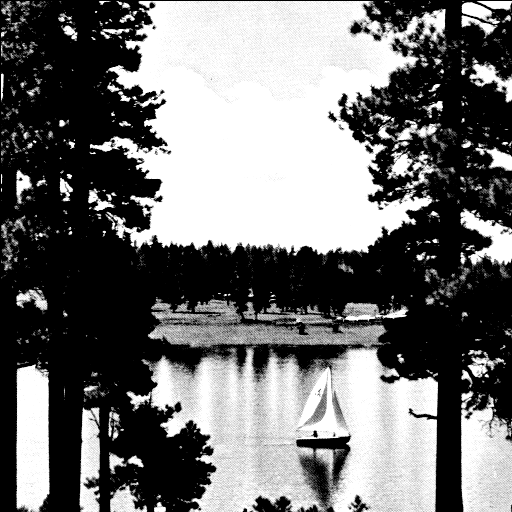
\includegraphics[width=0.5\textwidth]{./images/interpolation1.png}}
  \subfigure[Interpolation sinusoïdale]{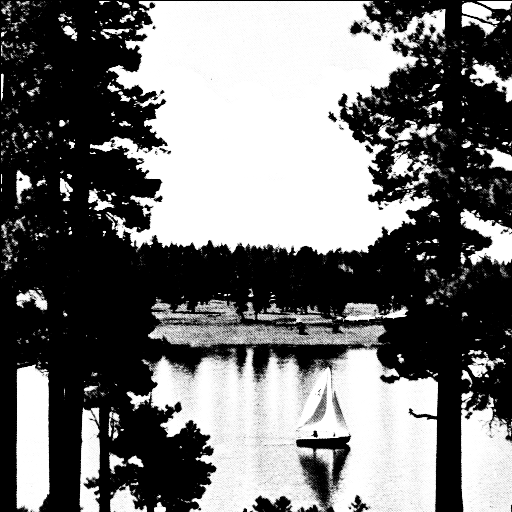
\includegraphics[width=0.5\textwidth]{./images/interpolation2.png}}
  \caption{Résultats}
\end{figure}
 
\FloatBarrier

\clearpage
\section{Conclusion}
Ces traitements sont plutôt simples à mettre en place, à l'exception des plus mathématiques, et permettent des modifications immédiatement visibles et compréhensibles. Le traitement d'images en couleur n'est pas plus complexe, il nécessite seulement de traiter séparément les composantes de l'image pour chaque pixel qui la compose.

\section{Remarques personnelles}
Ayant utilisé le language C auparavant, aussi bien en cours que dans mon temps libre, la mise en place du TP ne m'a pas posé problème. J'ai trouvé les exercices intéressants, compréhensibles et de difficulté croissante. J'ai également apprécié la possibilité de réaliser des exercices facultatifs, qui m'ont permis d'aller plus loin dans la compréhension des traitements d'images.

Vous pouvez trouver le code source de ce rapport et des programmes utilisés ici: \url{https://github.com/nfiacsan/S6/tree/main/Multimedia/image1}
\end{document}
